\documentclass[a4paper]{article}

\usepackage[english]{babel}
\usepackage[utf8]{inputenc}
\usepackage{mathtools}
\usepackage{gensymb}
\usepackage{verbatim}
\usepackage{amssymb}
\usepackage{amsmath}
\usepackage[thmmarks,amsmath]{ntheorem}
\usepackage{booktabs,siunitx}
\usepackage{graphicx}
\usepackage[colorinlistoftodos]{todonotes}
\usepackage{geometry}
\usepackage{float}
\usepackage{hyperref}
\usepackage{caption}
\usepackage[bottom]{footmisc}
\geometry{
 a4paper,
 total={170mm,257mm},
 left=30mm,
 right=30mm,
 top=20mm,
 }
\author{[[Name]]}
\title{Report - [[Experiment]]}

\begin{document}

% section hkdhgkjh (end)

\maketitle
\abstract 
The difference between a NaI detector and a Germanium detector are investigated in this experiment. It was found that the NaI detector is more efficient in detecting high energies, whereas the HPGe detector is more efficient in lower energies. The HPGe detector has a better resolution as well. Both systems were linear in detection of energies compared to their internal scale, but the error in system linearity in much smaller in the HPGe detector than in the NaI(TI) detector. The used sources were $^{137}Cs$, $^{152}Eu$, $^{207}Bi$, $^{22}Na$ and $^{60}Co$. Caesium and Europium were used to calibrate the energy scale.

The inverse square law for the dose rate of electromagnetic radiation was verified and concluded that the whole experiment took place within legal limits.

\section{Introduction}

To detect gamma rays, there are different detectors with different tradeoffs. Two of the most used detectors in gamma spectroscopy are discussed below.

\subsection{The NaI detector}

In this experiment a scintillator detector was used (see figure \ref{fig:setup}, label $5$). It had dimensions $1 '' \times 1.25 ''$. A scintillator is a material that emits light, when excited over radiation that carries enough energy to knock out electrons from atoms. The incoming energy is absorbed and emitted as photon. The luminescence falls exponentially depending on the fading time $\tau$, which is a characteristic quantity of the radioactive isotopes. The emitted photons hit a photomultiplier arranged directly after the scintillator material. The photomultiplier translates the emitted light into an electric impulse. Inside the device the photon knocks an electron out (photoelectric effect) of the photocathode. This electron is accelerated via an electric field, thus gains higher energy. The electron emits over secondary emission on a dynode multiple other electrons, which are accelerated again. This procedure is repeated, until there is enough energy to detect the pulse \cite{flyckt2002}. Since the photomultiplier amplifies linearly \cite{lush1965} and the scintillator emits light with amplitude proportional to the $\gamma$-quantum energy emitted from the source, we can deduce the gamma-energy, once we know the linear factor between the amplitude of the pulse and the gamma-energy.
\newline
The used scintillator material is Sodium iodide (NaI) with Thallium (TI) as activator. The fading time of NaI(TI) is around $250$ ns \cite{instruction_sheet}. This is small compared to other scintillator materials, but long enough to detect the emitted pulse.

\subsection{The HPGe detector}

The other detector used in this experiment is a semiconductor detector (see figure \ref{fig:setup}, label $4$). It was a Canberra GX1518 CP5-PLUS-SL (diameter $54$ mm, length $30.5$ mm) \cite{datasheet}. The used semicondcutor material is Germanium. In this detector the excitation of the crystal is also used to detect the energy. The needed energy to excite the crystal is far lower than in scintillator materials. The detector has thus a better resolution. Excitation inside the crystal produces free electrons and holes. The number of electron-hole pairs is proportional to the energy of the radiation to the semiconductor \cite{wiki:semi:2018}. With usage of an electric field the electron and holes are accelerated and thus create an electron pulse, which can be translated to a signal. To measure the amount of energy, the number of electron-hole-pair must be measured \cite{knoll1999}. HPGe stands for high purity germanium detector. The crystal needs to be as pure as possible, because impurities would trap the electrons and holes preventing them from accelerating and therefore degrade the performance of the detector. The operating temperature of the crystal also needs to be in the range of liquid nitrogen ($77^{\circ}K$). This is needed, because the electron can cross the band gap energy, but we want that they cross the band gap only when a gamma-ray excites it. This is one majoe drawback of HPGe detectors over scintillator detectors.

\subsection{Pulse-height analysis}

Subsequently after the detector (and the photomultiplier) the data was transferred to an 8k multi channel analyzer for processing. In this step the pulses are counted based on their amplitude. The different amplitudes correspond to the different channels. The channels were numbered from $0$ to $8191$, therefore in total $2^{13} = 8192$ channels. The reason why the multi channel analyzer used $13$ bits to encode the channels is probably a limitation of the bandwidth due to the cable or some internal boundary. However in a calibration step the channel scale has to be translated to an energy scale. The translation should be as linear as possible.

\section{Experimental setup}

To create comprehensive spectra, an array of devices is necessary. The detector is only one piece in the stack (see figure \ref{fig:setup} label ($4$) and ($5$)). Directly after the NaI detector, a photomultiplier is attached. From the protomultiplier, the signal is intensified using an amplifier, controlled over an oscilloscope and finally send to a multichannel analyzer, which was attached to a computer. The computer was used to analyze and visualize the recieved data. The HPGe detector was attached to the multichannel analyzer directly. In figure \ref{fig:setup} the whole experimental setup and its stack can be seen.

\begin{figure}[H]
\captionsetup{singlelinecheck=off}
\centering
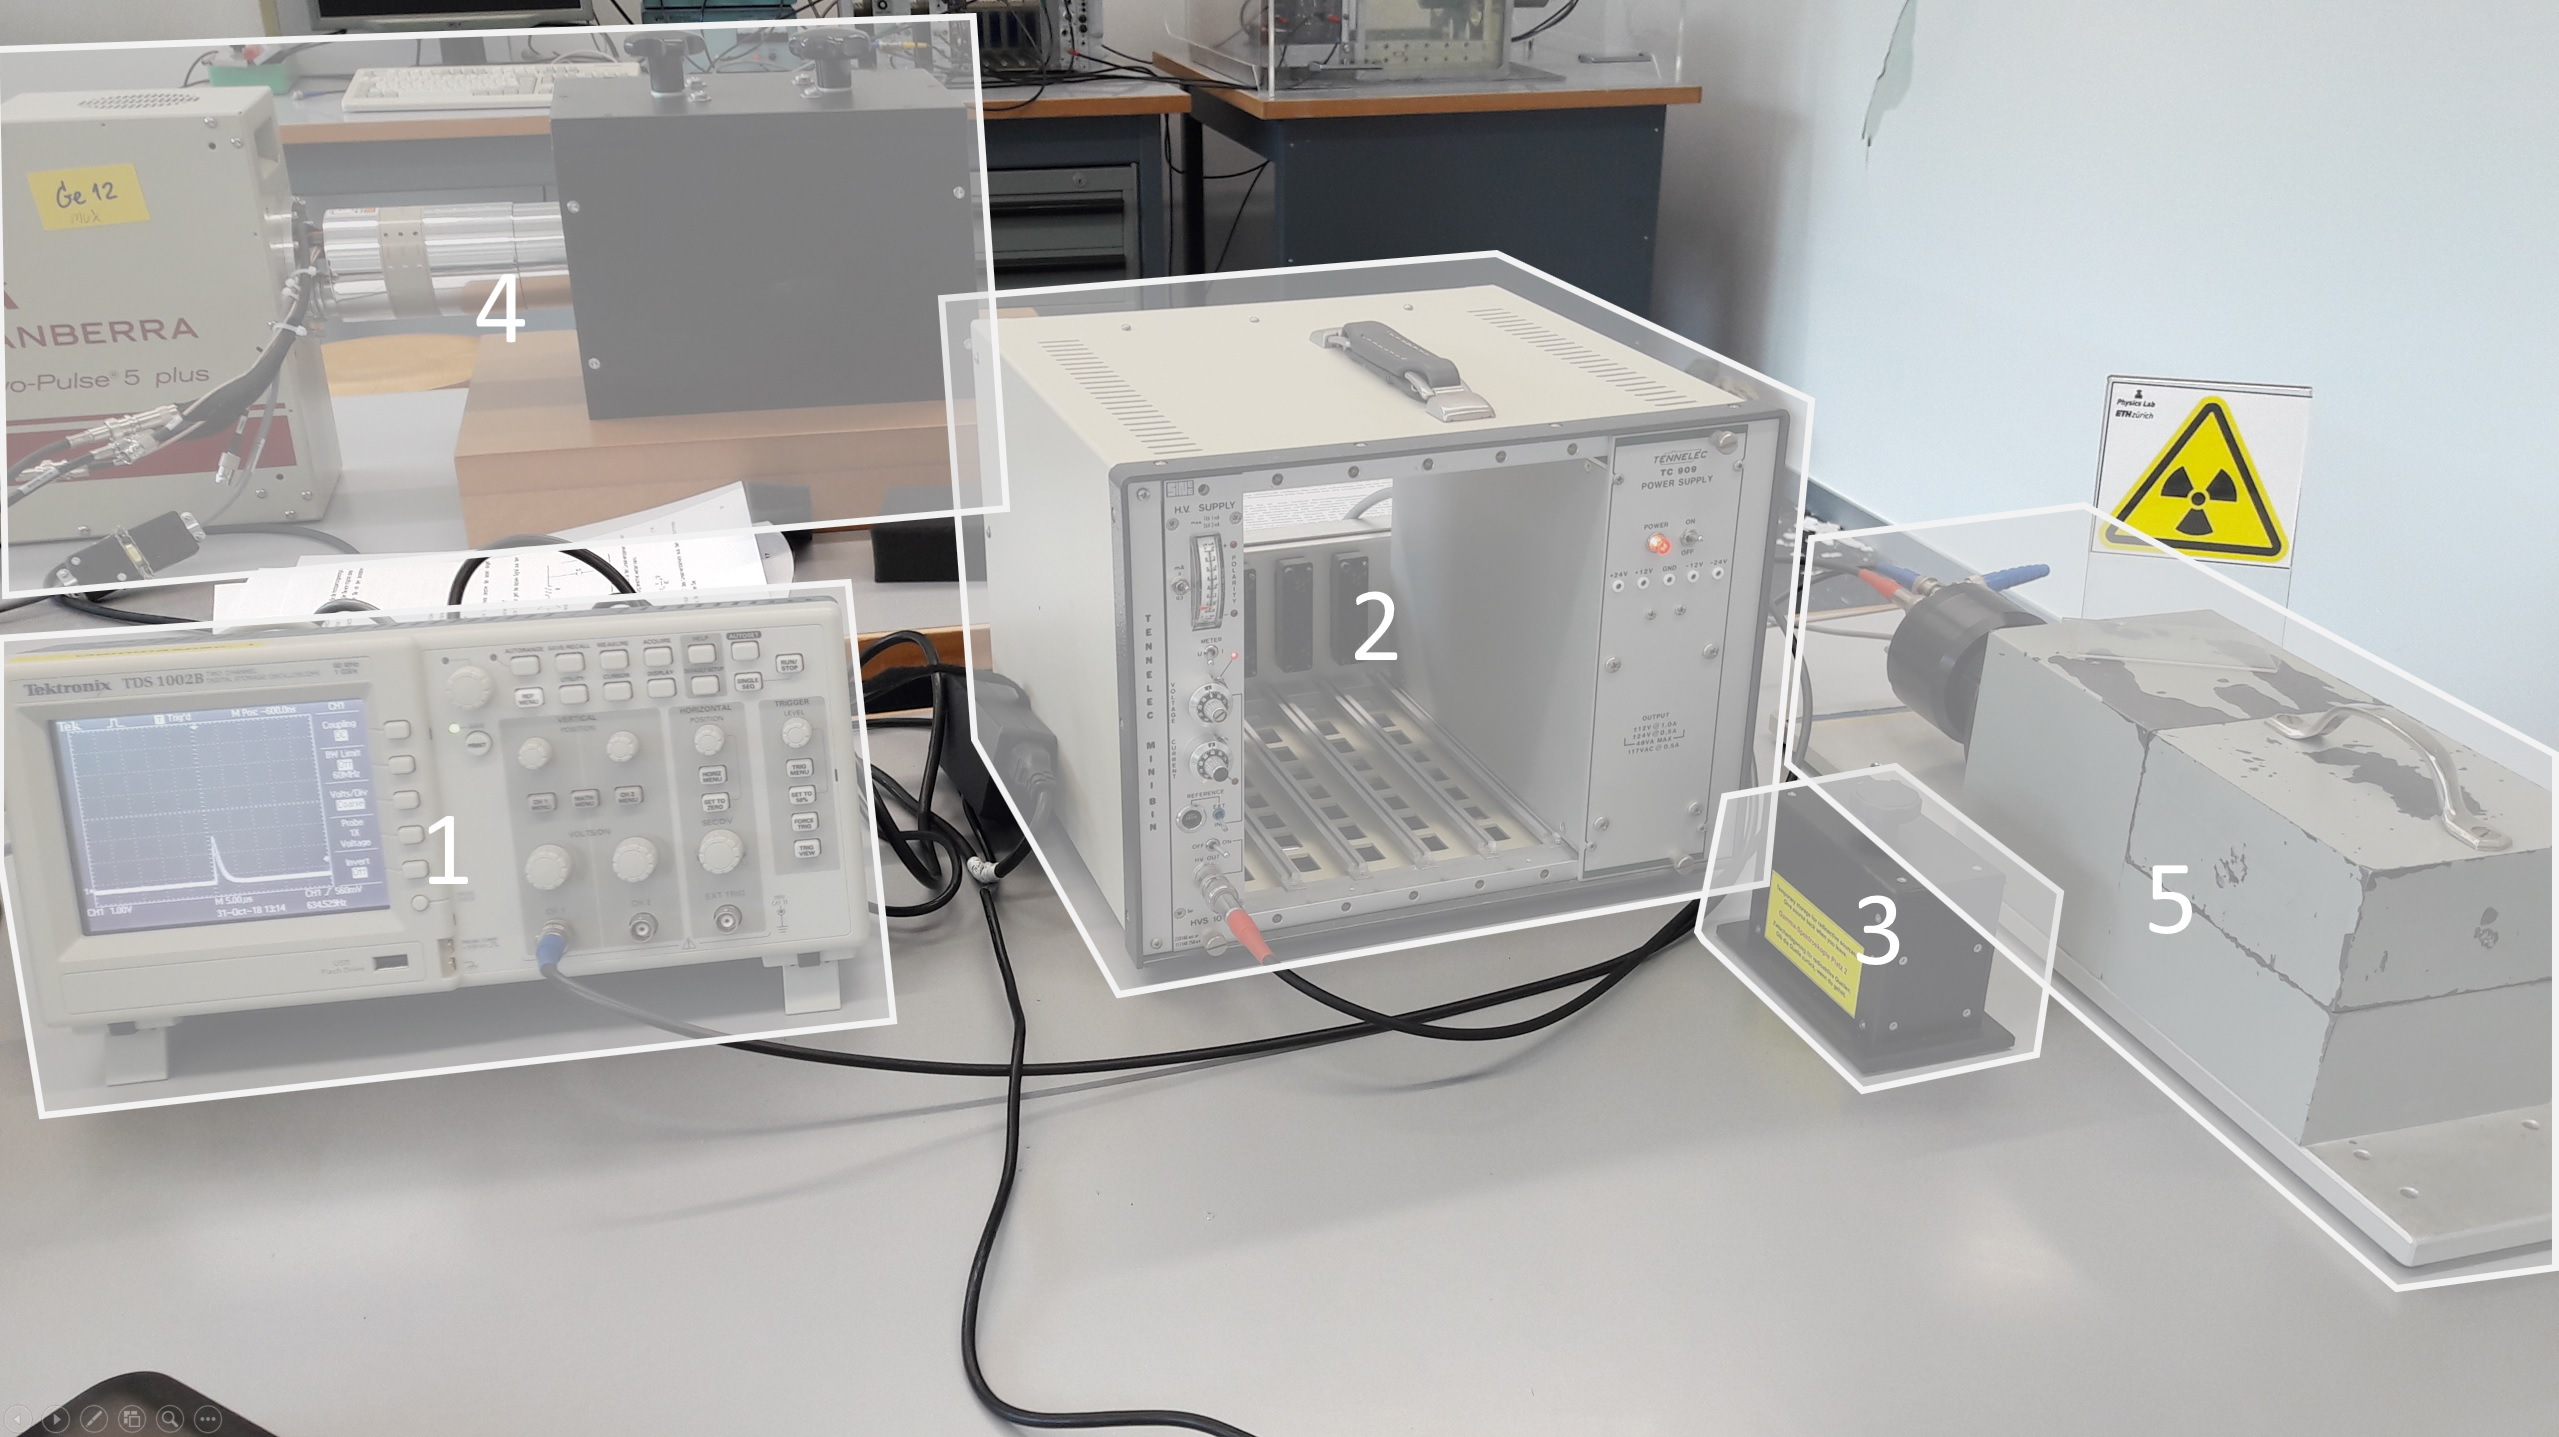
\includegraphics[width=1.0\textwidth]{img/setup.jpg}
\caption[blubb]{Image of the experimental setup. The device on the left ($1$) is the oscilloscope to visualize the pulse. $2$ is the amplifier of the signal coming from the photomultiplier behind the NaI detector ($5$). The amplifier is connected to a computer (not in the picture) to process the signal. In the background the HPGe (Germanium) detector ($4$) can be seen, which is directly connected to a computer (not shown). $3$ is the cannister to store the radioactive sources. Source: Authors' own.}
\label{fig:setup}
\end{figure}

Post processing to the data was done using a computer programm called MCDWIN \cite{mcdwin:2018} shipped in combination with the multichannel analyzer. The progamm generates text files from the incoming data. These text files contained a mapping of the $8192$ channels and the number of incidents happend in that channel. By "incidents", the number of gamma-quantums with energy corresponding to the channel is meant.

\subsection{Energy calibration}

To translate the channel scale to a energy scale, the application needed to be calibrated first. This was done using a known source - a $^{137}Cs$-source. We know that the cesium source should have a peak at around $662.61$ keV of intensity $84.62 \%$ according to the instruction sheet \cite{instruction_sheet} (table in section A.4). To calibrate the scale of the application, we measured the spetrum of the known cesium source and successively identified the photo peak at $662.61$ keV. Setting channel number $0$ to $0$ keV, we can now perform a linear interpolation of these $2$ points, giving a linear translation from the channel scale to an energy scale in keV. This was done using the other sources and their known peaks too, recieving a better precision in translation of channels to keV. With this calibration, the spectra of all the sources can be recorded.

\subsection{Efficiency calibration}

The efficiency is defined as the ratio of the number of counts recorded by the detector to the number of radiation emitted by the source \cite{akkurt2014}. In a formula this would be:

\begin{equation}
\mathcal{E} = \frac{A_{now} \frac{\Omega_D}{4 \pi} }{ \frac{N_{photo}}{ \varepsilon(E_{\gamma}) } }
\label{eq:eff}
\end{equation}

where $A_{now}$ is the activity of the source right now, $\Omega_D$ is the solid angle of the detector, $N_{photo}$ is the intensity of the photo peak at energy $E_{\gamma}$ and $\varepsilon(E_{\gamma})$ is the absorbtion probability from \cite{instruction_sheet} table A1.

\subsection{Measurement Method}

For each source, the spectrum was recorded. After the source was placed in front of the detector, the computer programm was set up to start the recording of the data. The duration of recording depended on how distinctly and visibly the expected photo peaks were in the live generated spectrum plot. In some cases, it was necessary to change the scale in y-direction (counts) to a logarithmic scale to be able to see the peaks. This was in most cases applied to the spectra plots included in this report. When the spectra were comprehensive enough to study, the application was stopped, the data saved to an external file and a new source was attached into the mount.

\subsection{Dose rate}
In a first step a verification of the inverse square law for the dose rate of electromagnetic radiation was done. For this, the known cesium source was taken and the radiation in $\mu Sv / hr$ was measured using a measuring device. This was done in small steps of distance starting from $0$ m to $\sim 1$ m.

\section{Results and Discussion}

\subsection{Dose rate}
\label{sec:doserate}

In figure \ref{fig:dose_rate}, the measured data and its inverse square fit are plotted, where in y-direction the radiation dose in $\mu Sv / hr$ and in x-direction the distance to the source from $0$ to one meter is plotted. It can be seen that - according to the measurements - the dose rate behaves like the inverse square law, with the fit function approximating the data quiet well (see table \ref{tab:doserate} for all measured data).

\begin{figure}[H]
\centering
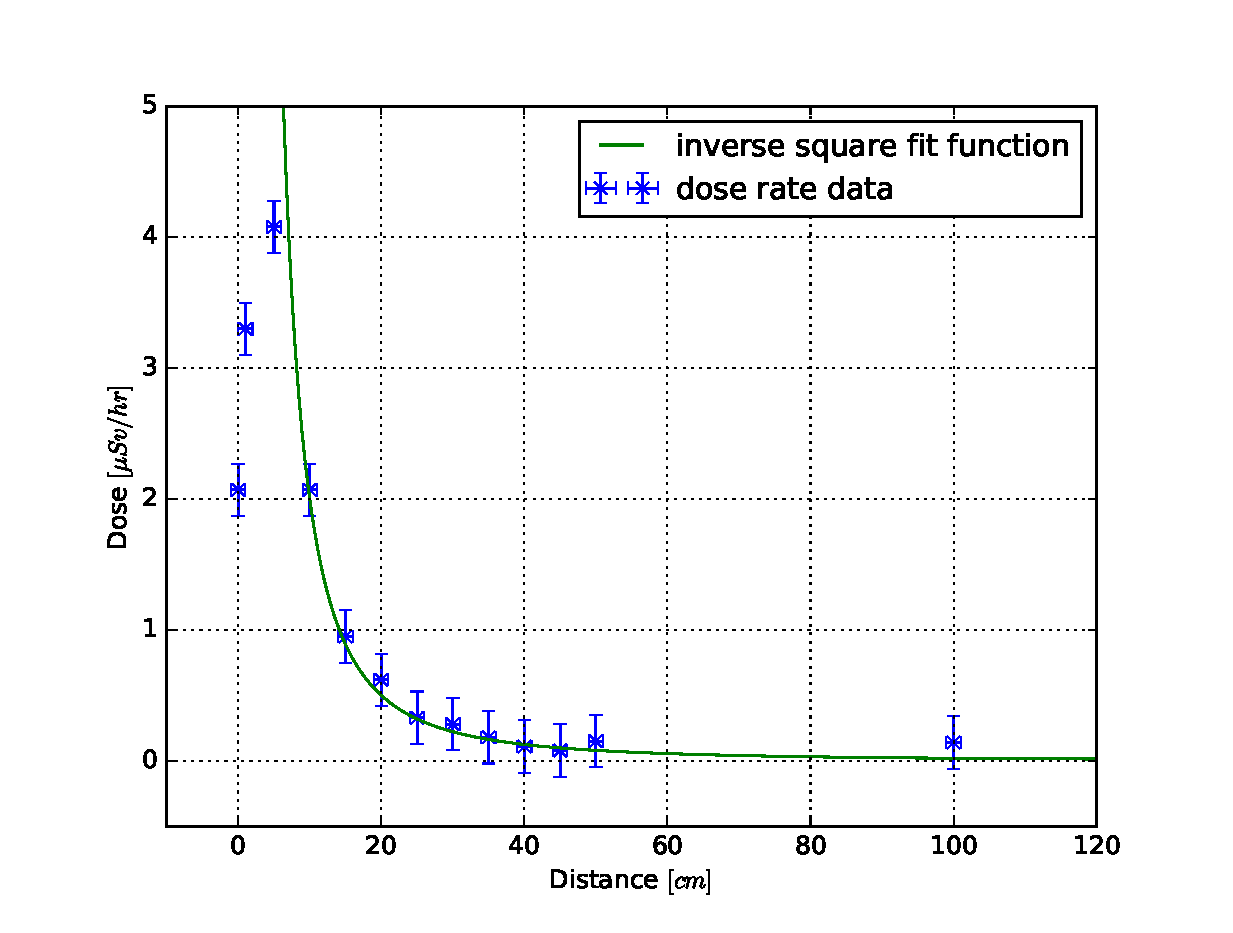
\includegraphics[width=1.0\textwidth]{plots/dose_rate.eps}
\caption{Plot of the dose rate of the $^{137}Cs$-source. The inverse square fit: $f(x) = a \cdot x^{-2}$ with $a = [[fit:a]]$. Source: Authors' own.}
\label{fig:dose_rate}
\end{figure}

In Switzerland, the effective dose rate that must not be exceeded is $1 \, mSv / year$ \cite{strahlenschutzverordnung}. If we take the value of $4 \, \mu Sv / hr$ (which is only if we stay very close to the bare source - say $\sim 5 \, cm$), we would be able to stay there for $250$ hours to gain an exposure of $1 \, mSv$. During the whole experiment, the sources were exposed to us for $\sim 5$ minutes in total. This gives a dose of $0.33 \, \mu Sv$. Therefore the dose we recieved during this experiment is far below the legal limit.

\subsection{Activity}

In a second step the activity of the known sources should be measured and compared to the activity gained trough the radioactive decay law. The activity of the known $^{137}Cs$ source was $A_{then} = [[A_then]] \, kBq$ at the date $1.4.2000$ and the calculated activity today (according to the law of radioactive decay) is

\begin{equation}
A_{now,calc} = A_{then} \exp{\left( -\frac{t}{\tau} \right)} = [[A_now]] \, kBq
\label{eq:decay_law}
\end{equation}

where $\tau = \frac{t_{1/2}}{\ln{\left( 2 \right)}}$ is the the average lifetime of a radioactive particle before decay, $t_{1/2} = 30.1 \, y$ is the half-life time of $^{137}Cs$ and $t$ is the time in seconds since $1.4.2000$.

On the other side, the measured activity of the $^{137}Cs$ source is calculated with the following formula:

\begin{equation}
A_{now,meas} = \frac{N_{Photo}}{\frac{\Omega}{4 \pi} \varepsilon(E_{\gamma}) \Gamma(E_{\gamma}) \omega(E_{\gamma})} = [[A_meas]] \, kBq
\label{eq:activity_meas}
\end{equation}

where $E_{\gamma}$ is the energy of the peak at $661.62 \, keV$ of the known $^{137}Cs$ spetrum, $\Gamma(E_{\gamma})$ is the peak/total ratio of the NaI detector gained from the instruction sheet (figure A2, graph for $1" \times 1"$, since our detector has dimensions $1.25" \times 1"$) for the given $E_{\gamma}$ and $\omega(E_{\gamma})$ is the intensity of the peak, also given on the instruction sheet in section A.4 \cite{instruction_sheet}.
The used quantities for this formula were:

\begin{subequations}
\begin{align}
E_{\gamma} &= [[E_gamma_cs]] \, keV \\
\Gamma(E_{\gamma}) &= [[Delta]] \\
\omega(E_{\gamma}) &= [[emission_prob]] \\
\Omega \cdot \varepsilon(E_{\gamma}) &= [[omega_eps]] \\
\mu_{NaI}(E_{\gamma}) &= [[mu_NaI]] \\
\mu_{Pb}(E_{\gamma}) &= [[mu_Pb]] \\
\varepsilon_{NaI}(E_{\gamma}) &= [[eps_NaI]] \\
\Omega &= [[omega_D]] \, sr
\label{eq:activity_quantities}
\end{align}
\end{subequations}

The activities of the other sources were calculated in the same way using the areas under the corresponding peaks as intensities of the photo peaks. In table \ref{tab:activites} the calculated activities for each recognizable peak of the known sources are listed.

\begin{table}[H]
\centering
\caption{Activities of the sources calculated over their photo peaks using the NaI detector.}
\begin{tabular}{rr|rr}
\hline
[[table:activities]]
\end{tabular}
\label{tab:activites}
\end{table}

\subsection{System Linearity}

A further very important property of detectors is their linearity in energy. Figure \ref{fig:system_linearity} displays a plot of the internal scale (channels) to the translated energy scale (in keV). For this, all the photopeaks that were recognizable, were plotted with their gamma-energy against their value in channels. For an ideal detector this should be a perfect line going trough $0$ at $0$ eV. It can be seen that the NaI detector (left) has an offset of $[[linear_fit_NaI:b]]$ channels. This means that at $0$ eV energy the channel number is still $[[linear_fit_NaI:b]]$, where on the other side the HPGe detector (right) has on offset of just $[[linear_fit_HPGe:b]]$ channels. It is also worth to recognize that the error in the linear coefficient is much smaller for the HPGe detector than for the NaI detector. ($[[linear_fit_HPGe:a_err]]$ compared to $[[linear_fit_NaI:a_err]]$)
\newline
To conclude, the system linearity of the HPGe detector is much better than the linearity of the NaI detector.

\begin{figure}[H]
	\begin{minipage}[t]{0.5\textwidth}
		\begin{center}
		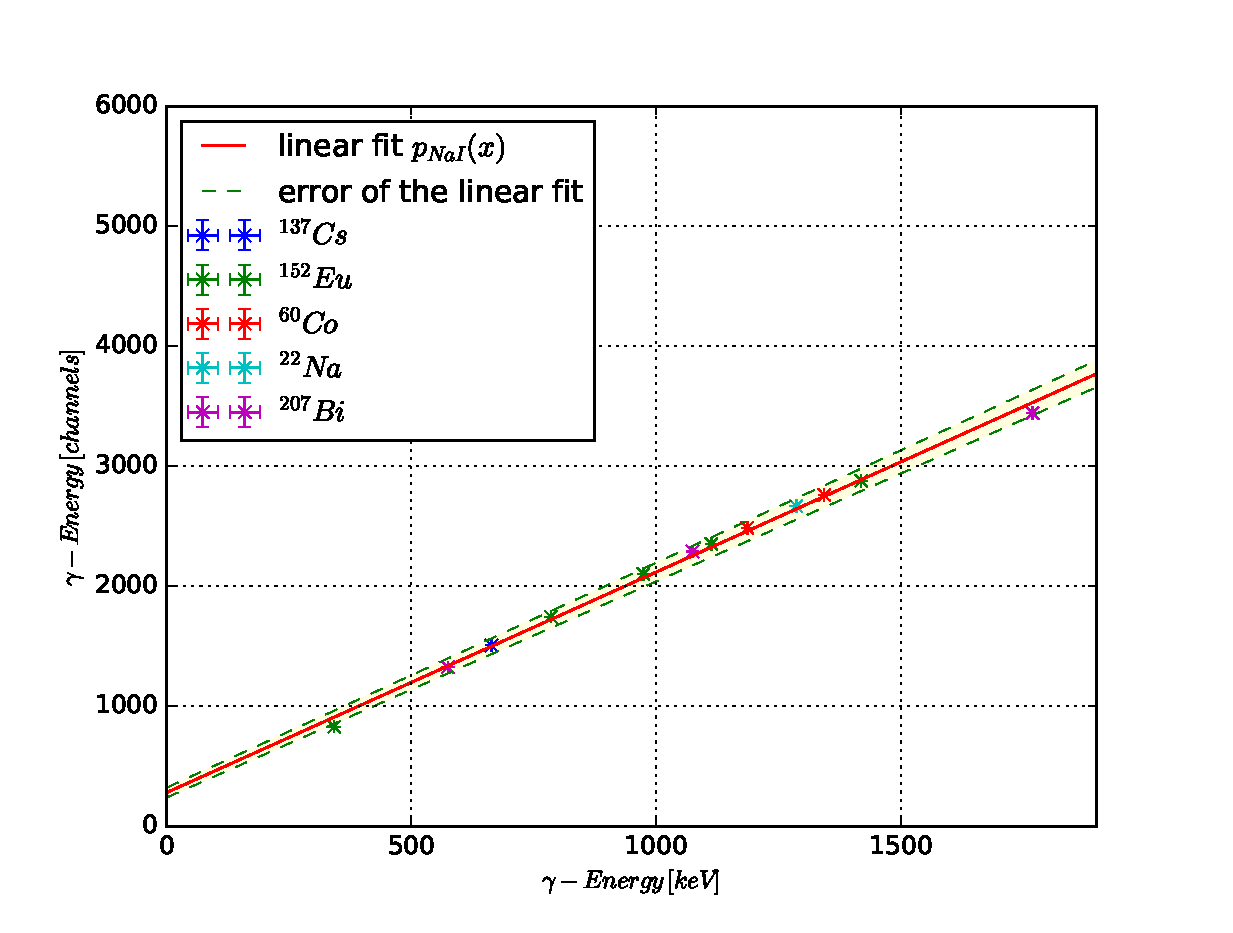
\includegraphics[width=1.0\textwidth]{plots/system_linearity_NaI.eps}
		\end{center}
	\end{minipage}
	\begin{minipage}[t]{0.5\textwidth}
		\begin{center}
		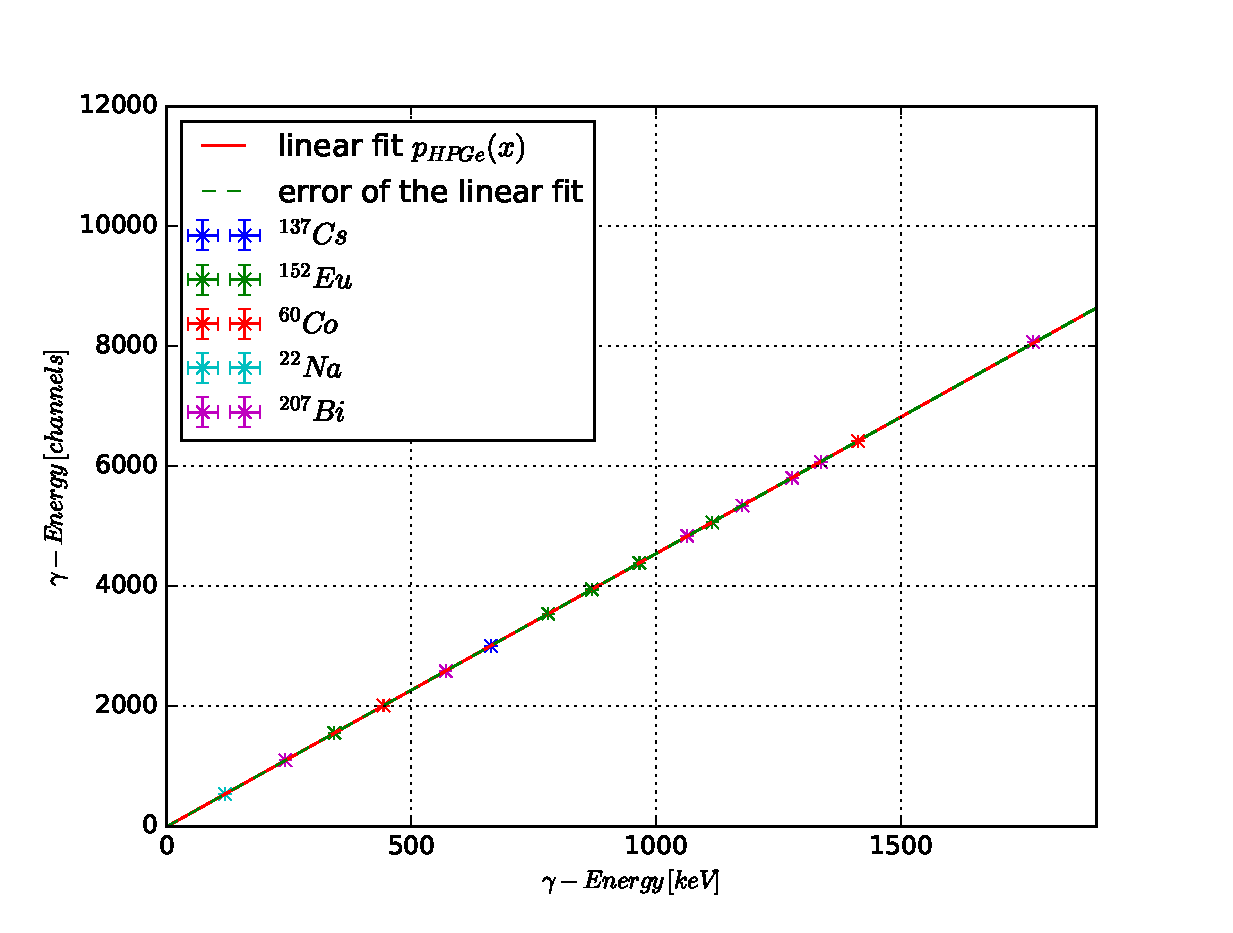
\includegraphics[width=1.0\textwidth]{plots/system_linearity_HPGe.eps}
		\end{center}
	\end{minipage}
	\caption{Linearity of the measurement system; left: $NaI$-detector, right: $Ge$-detector. The linear fit functions: $p_{NaI}(x) = [[linear_fit_NaI]]$ and $p_{HPGe}(x) = [[linear_fit_HPGe]]$. Source: Authors' own.}
	\label{fig:system_linearity}
\end{figure}

\subsection{Efficiency}

Using the definition of efficiency from above \eqref{eq:eff}, the efficiency of the NaI detector for the $^{137}Cs$ source at the photopeak ($662.61$ keV) with respect to the solid angle was calculated to be $[[efficiency]] \, \%$ (the value of \eqref{eq:decay_law} was taken for the activity). This result is in the usual area for scintillator detectors and seems to be plausible according to literature values of NaI scintillator detectors \cite{hossain2011}. For the efficiencies of the other sources refer to table \ref{tab:efficiencies}. Note that the efficiency for $^{137}Cs$ is not the same as in the text above. The reason is that the value of \eqref{eq:activity_meas} was taken to calculate the activity used in the calculation of the efficiency.

\begin{table}[H]
\centering
\caption{Efficiencies of the sources calculated over their photo peaks using the NaI detector.}
\begin{tabular}{rr|rr}
\hline
[[table:efficiencies]]
\end{tabular}
\label{tab:efficiencies}
\end{table}

\subsection{Relative Resolution}

In the analysis of detectors in gamma spectroscopy, the relative resolution plays an important role. Figure \ref{fig:relative_resolution} displays relative resolution $\Delta E/E$ as a function of gamma ray energies $E_{\gamma}$ for the two detectors. According to literature \cite{hossain2011}, the measurements seem to agree. The relative resolution is much smaller in the HPGe detector (right) than in the NaI detector (left). Thus the NaI detector is more efficient, whereas the HPGe detector has a better resolution. One explanation for this could be that the excitation energy of germanium is much lower than for NaI ($2.84$ eV compared to $50$ eV). It can be seen that the resolution increases with higher energies (the lower the $\Delta E/E$ the better the resolution) and saturates for high enough energies, thus the exponential fit is justified. For the NaI detector, the measured data spreads widely, whereas the the data for the HPGe detector lie very close to the fit function.

\begin{figure}[H]
	\begin{minipage}[t]{0.5\textwidth}
		\begin{center}
		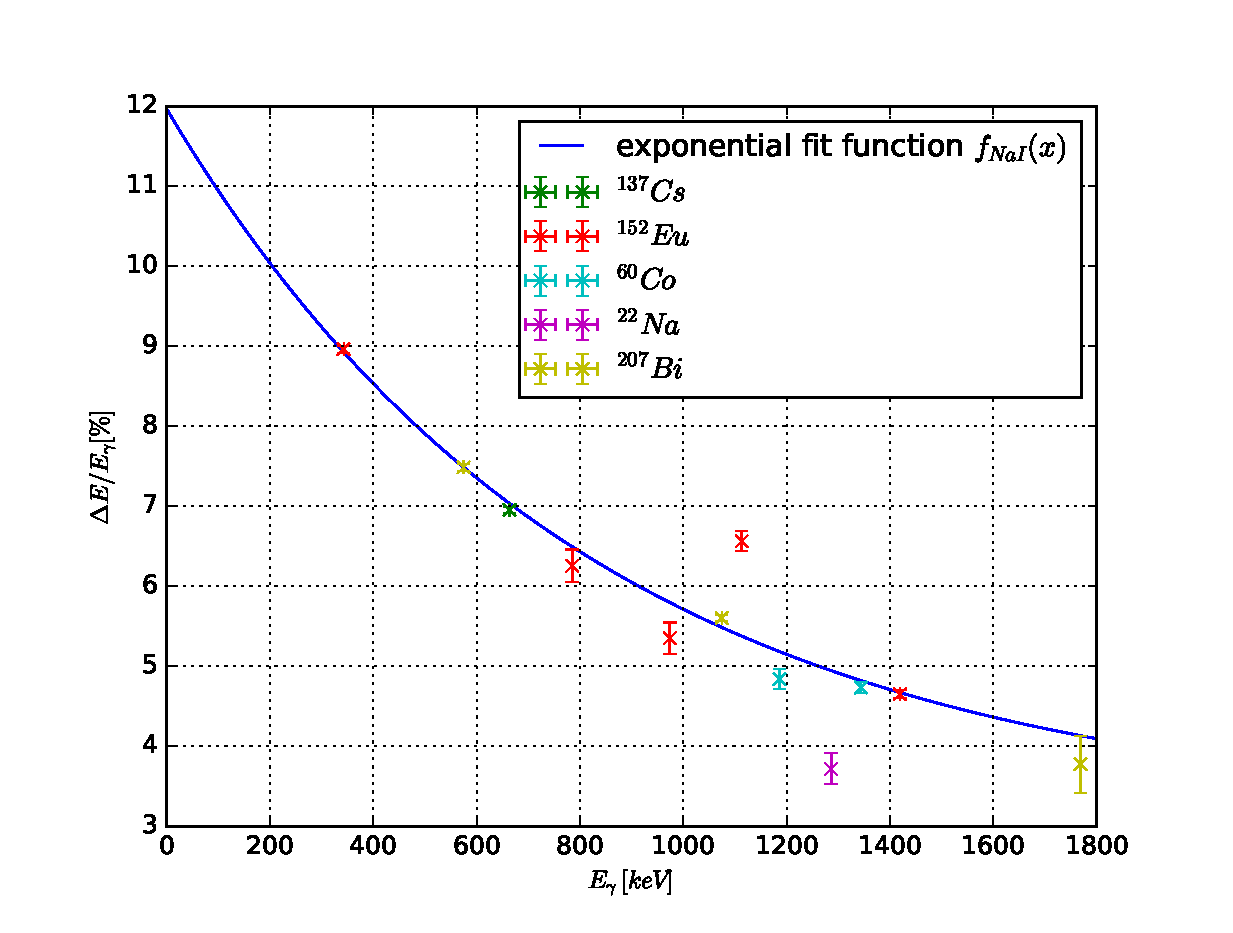
\includegraphics[width=1.0\textwidth]{plots/relative_resolution_NaI.eps}
		\end{center}
	\end{minipage}
	\begin{minipage}[t]{0.5\textwidth}
		\begin{center}
		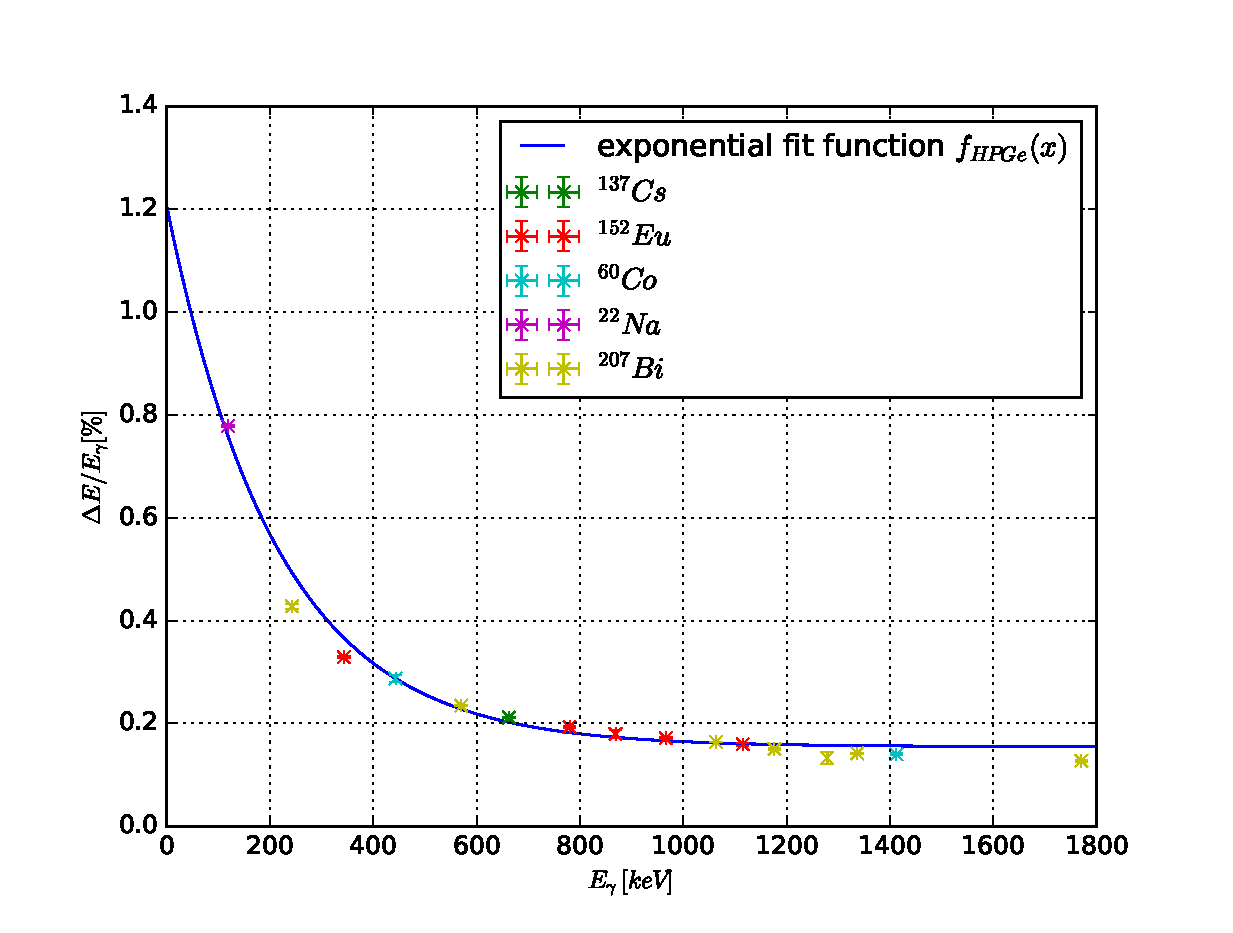
\includegraphics[width=1.0\textwidth]{plots/relative_resolution_HPGe.eps}
		\end{center}
	\end{minipage}
	\caption{Relative resolution power of the detectors; left: $NaI$-detector, right: $Ge$-detector. The exponential fit functions: $f_{NaI}(x) = a_{[[det:1]]} \cdot \exp \left( b_{[[det:1]]} \cdot x + c_{[[det:1]]} \right) + d_{[[det:1]]}$ and $f_{HPGe}(x) = a_{[[det:2]]} \cdot \exp \left( b_{[[det:2]]} \cdot x + c_{[[det:2]]} \right) + d_{[[det:2]]}$ with $a_{[[det:1]]} = [[a_det:1]]$, $b_{[[det:1]]} = [[b_det:1]]$, $c_{[[det:1]]} = [[c_det:1]]$, $d_{[[det:1]]} = [[d_det:1]]$ and $a_{[[det:2]]} = [[a_det:2]]$, $b_{[[det:2]]} = [[b_det:2]]$, $c_{[[det:2]]} = [[c_det:2]]$, $d_{[[det:2]]} = [[d_det:2]]$. Source: Authors' own.}
	\label{fig:relative_resolution}
\end{figure}

\begin{comment}
\begin{figure}[H]
\centering
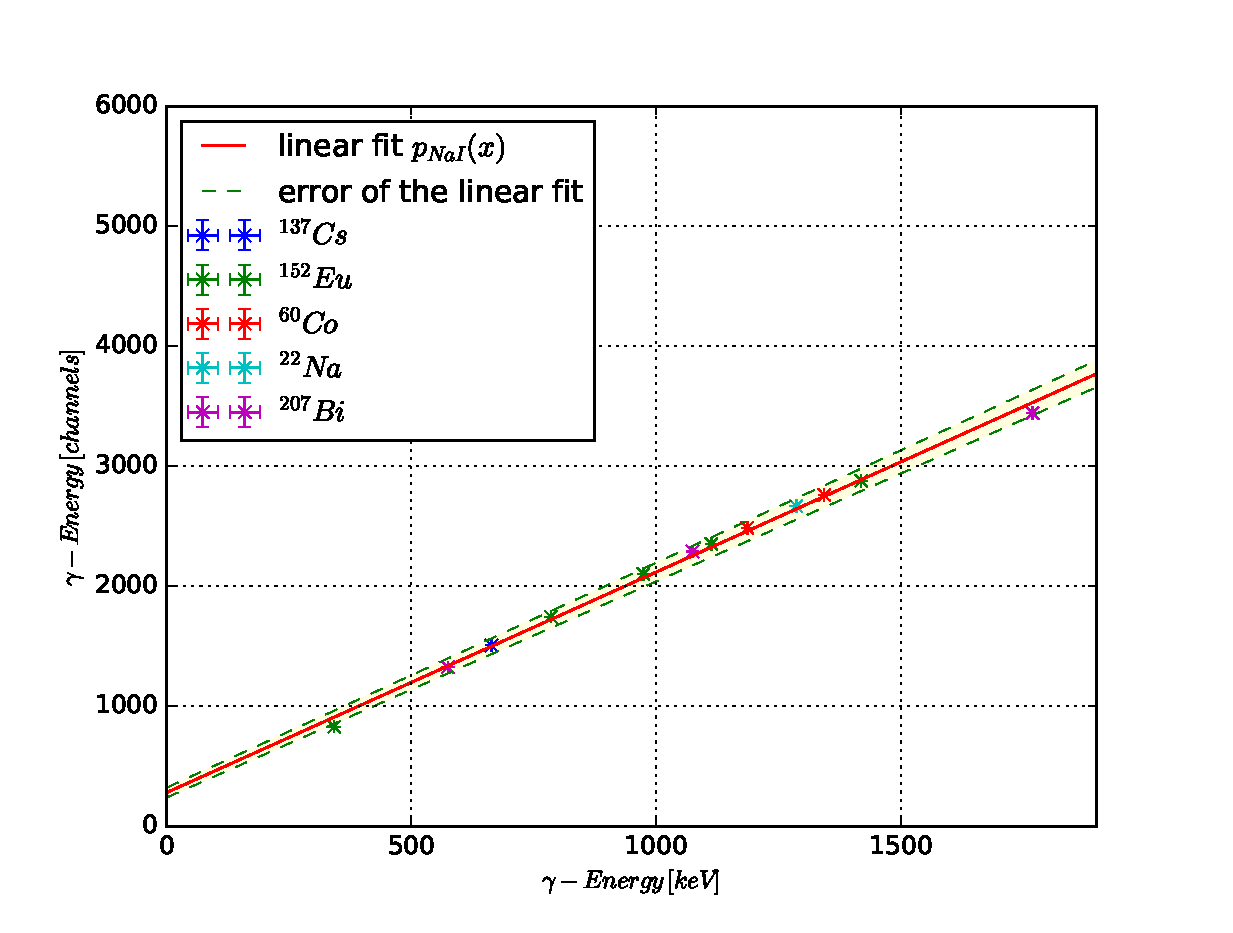
\includegraphics[width=1.0\textwidth]{plots/system_linearity_NaI.eps}
\caption{Linearity of the NaI measurement system. The linear fit: $p(x) = [[linear_fit_NaI]]$. Source: Authors' own.}
\label{fig:system_linearity_NaI}
\end{figure}

\begin{figure}[H]
\centering
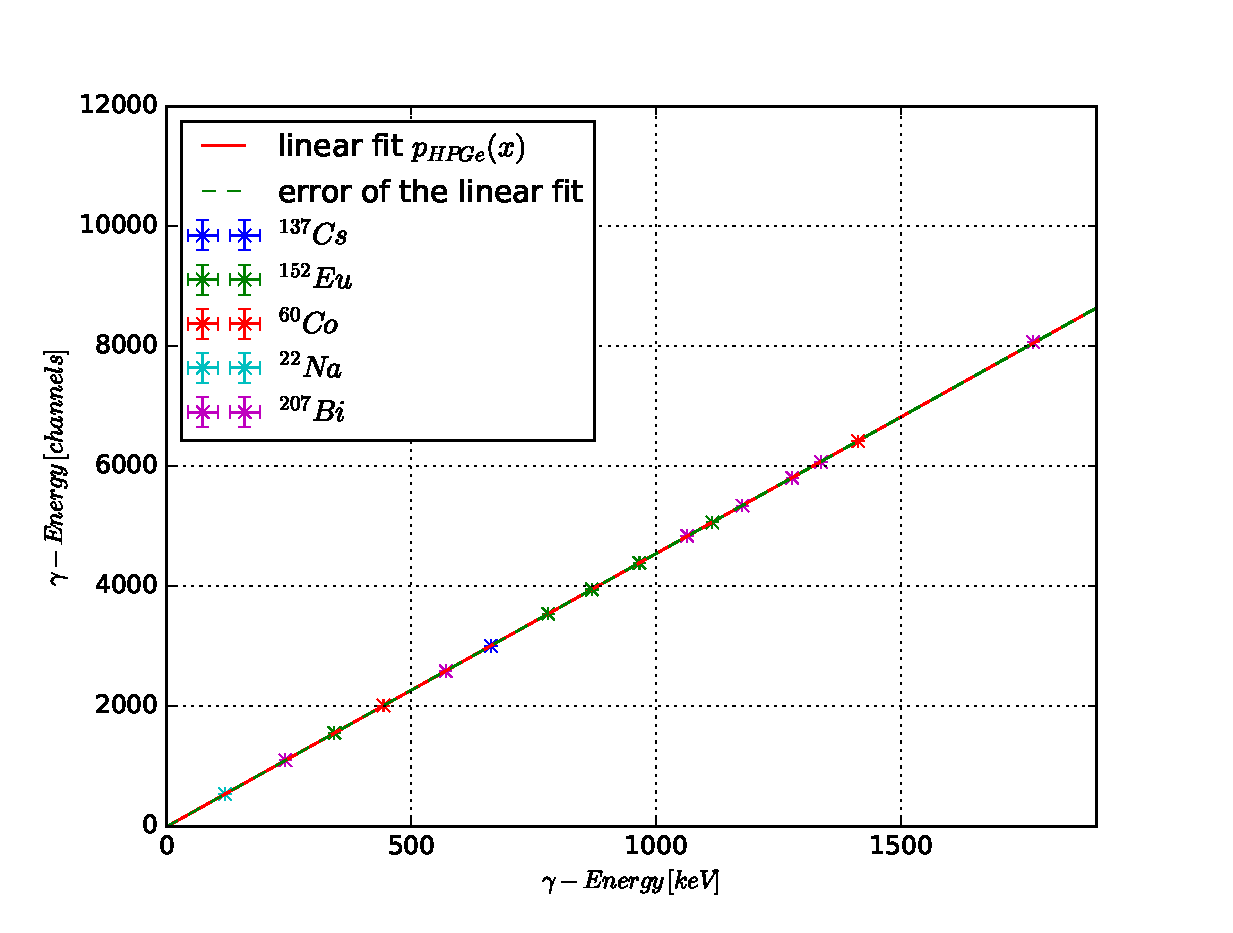
\includegraphics[width=1.0\textwidth]{plots/system_linearity_HPGe.eps}
\caption{Linearity of the HPGe measurement system. The linear fit: $p(x) = [[linear_fit_HPGe]]$. Source: Authors' own.}
\label{fig:system_linearity_HPGe}
\end{figure}

\begin{figure}[H]
\centering
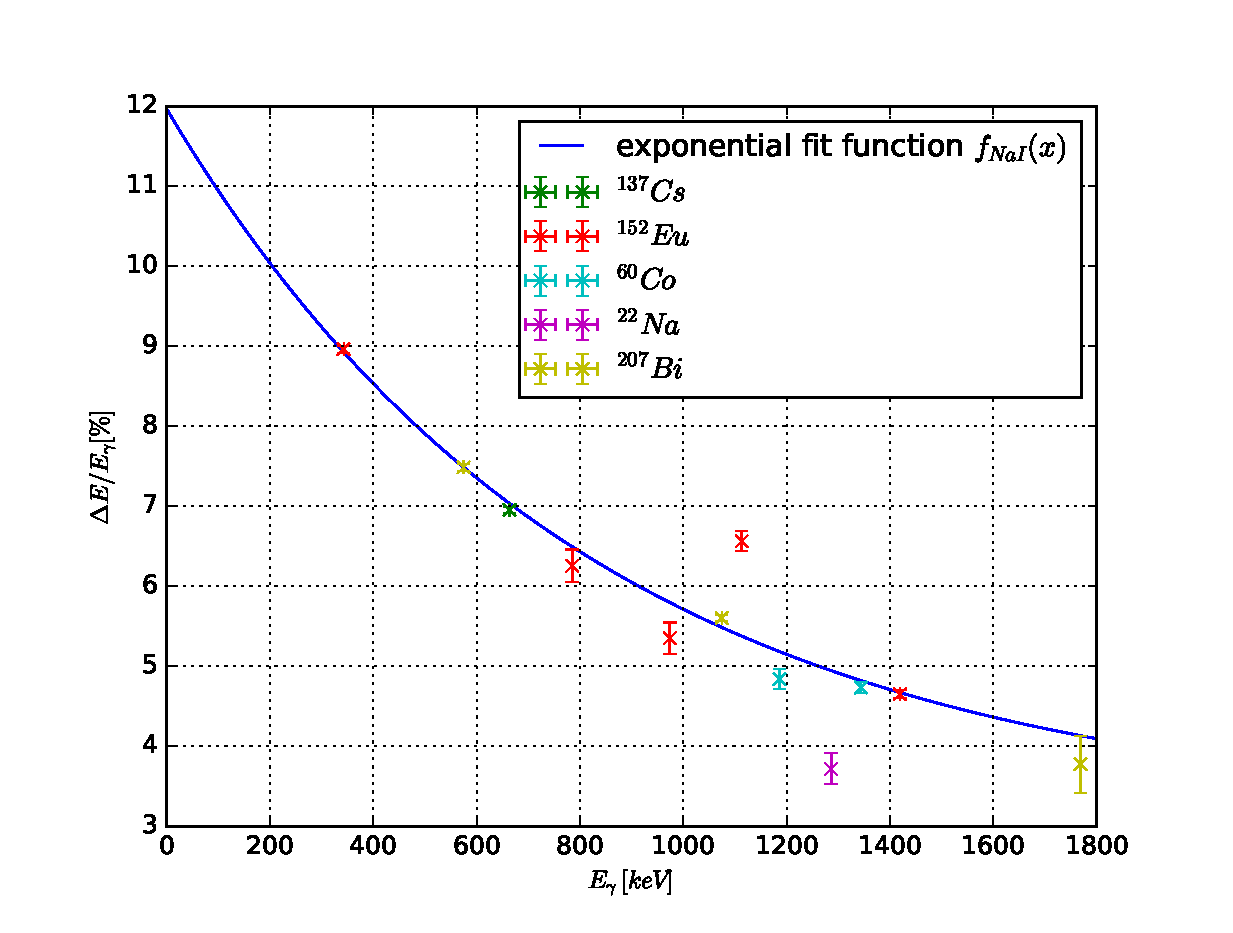
\includegraphics[width=1.0\textwidth]{plots/relative_resolution_NaI.eps}
\caption{Relative resolution power of the NaI-detector $\Delta E / E_{\gamma}$ against the Energy $E_{\gamma}$. Source: Authors' own.}
\label{fig:relative_resolution_NaI}
\end{figure}

\begin{figure}[H]
\centering
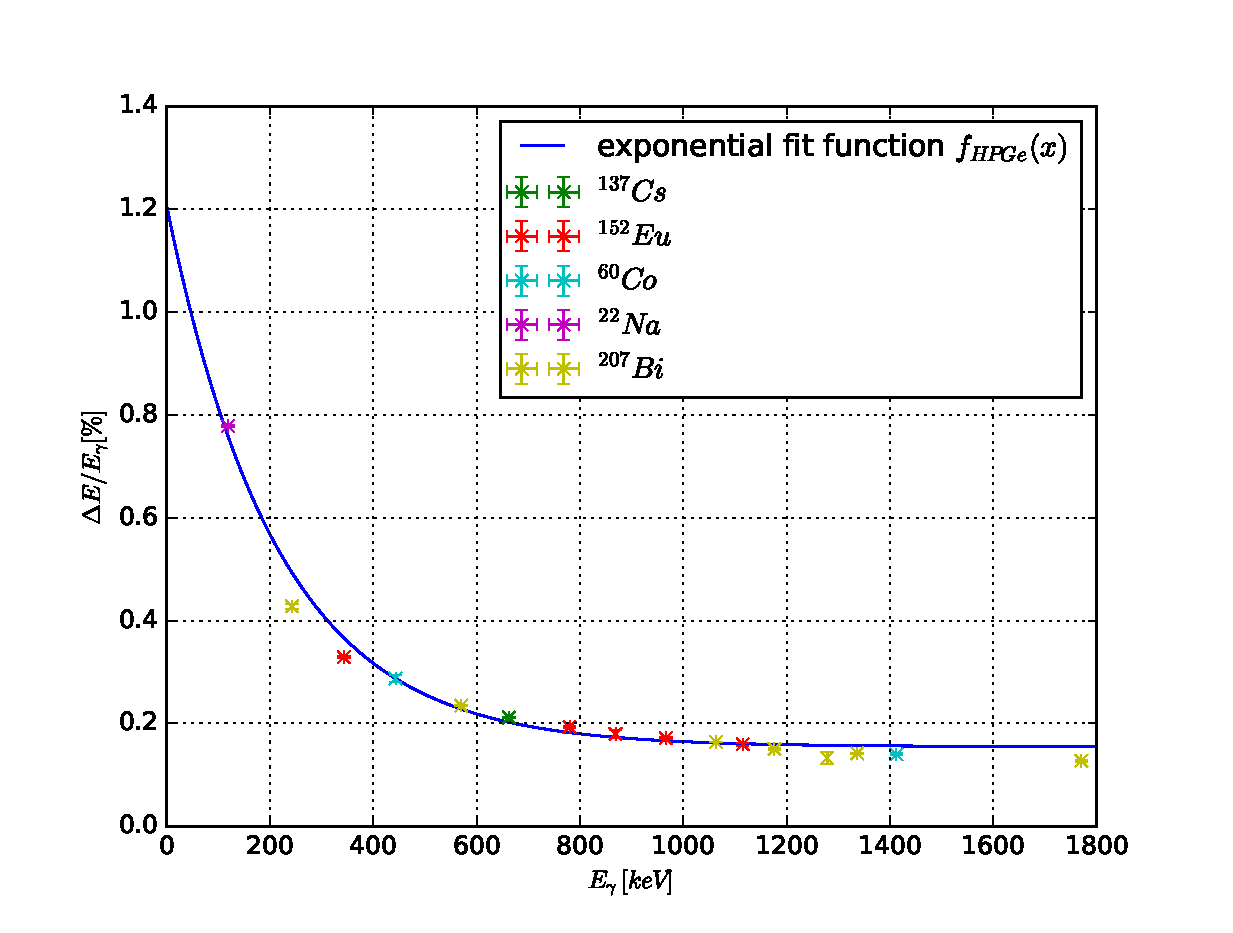
\includegraphics[width=1.0\textwidth]{plots/relative_resolution_HPGe.eps}
\caption{Relative resolution power of the HPGe-detector $\Delta E / E_{\gamma}$ against the Energy $E_{\gamma}$. Source: Authors' own.}
\label{fig:relative_resolution_HPGe}
\end{figure}
\end{comment}

\subsection{Analysis of the spectra for $^{137}Cs$}

As stated above, for the calibration of the application, a known cesium source was used. Figure \ref{fig:cs137} shows the resulting spectrum of that source. The peaks that were recognizable were annotated directly in the graph. Using the HPGe detector the spectrum was recored 3 times using different distances of the source to the detector ($1$ cm, $4$ cm  and $8$ cm). In all following spectra, blue is the spetrum for $1$ cm distance, green is $4$ cm and red $8$ cm respectively.
\newline
In both detectors, all interesting peaks can be recognized when investigating the graph. In the graph of the HPGe detector (right), we see that the closer the source is to the detector, the more intense is the radiation. This result goes consistent with the inverse square behavior of the dose rate (see section \ref{sec:doserate}).

\begin{figure}[H]
	\begin{minipage}[t]{0.5\textwidth}
		\begin{center}
		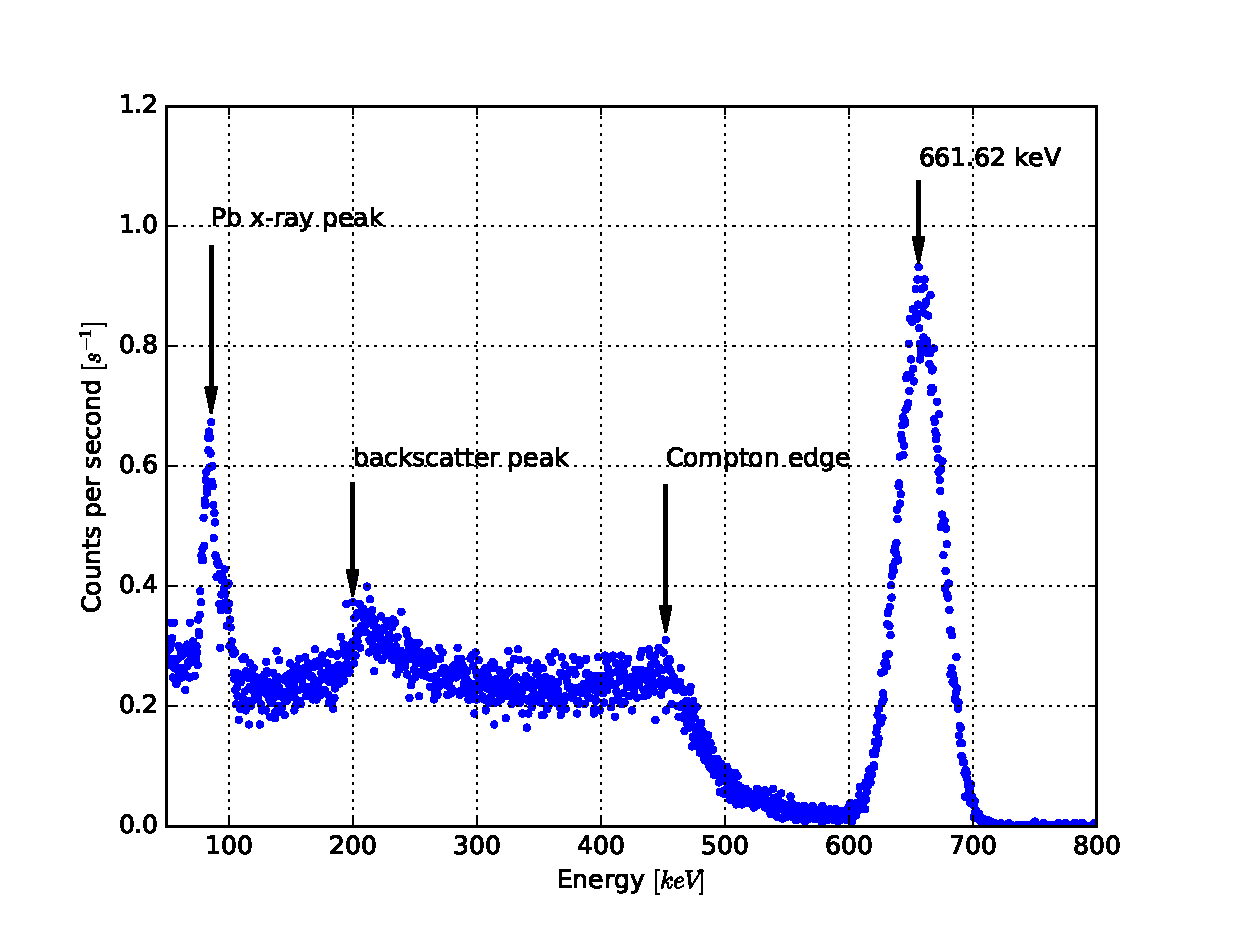
\includegraphics[width=1.0\textwidth]{plots/cs137.eps}
		\end{center}
	\end{minipage}
	\begin{minipage}[t]{0.5\textwidth}
		\begin{center}
		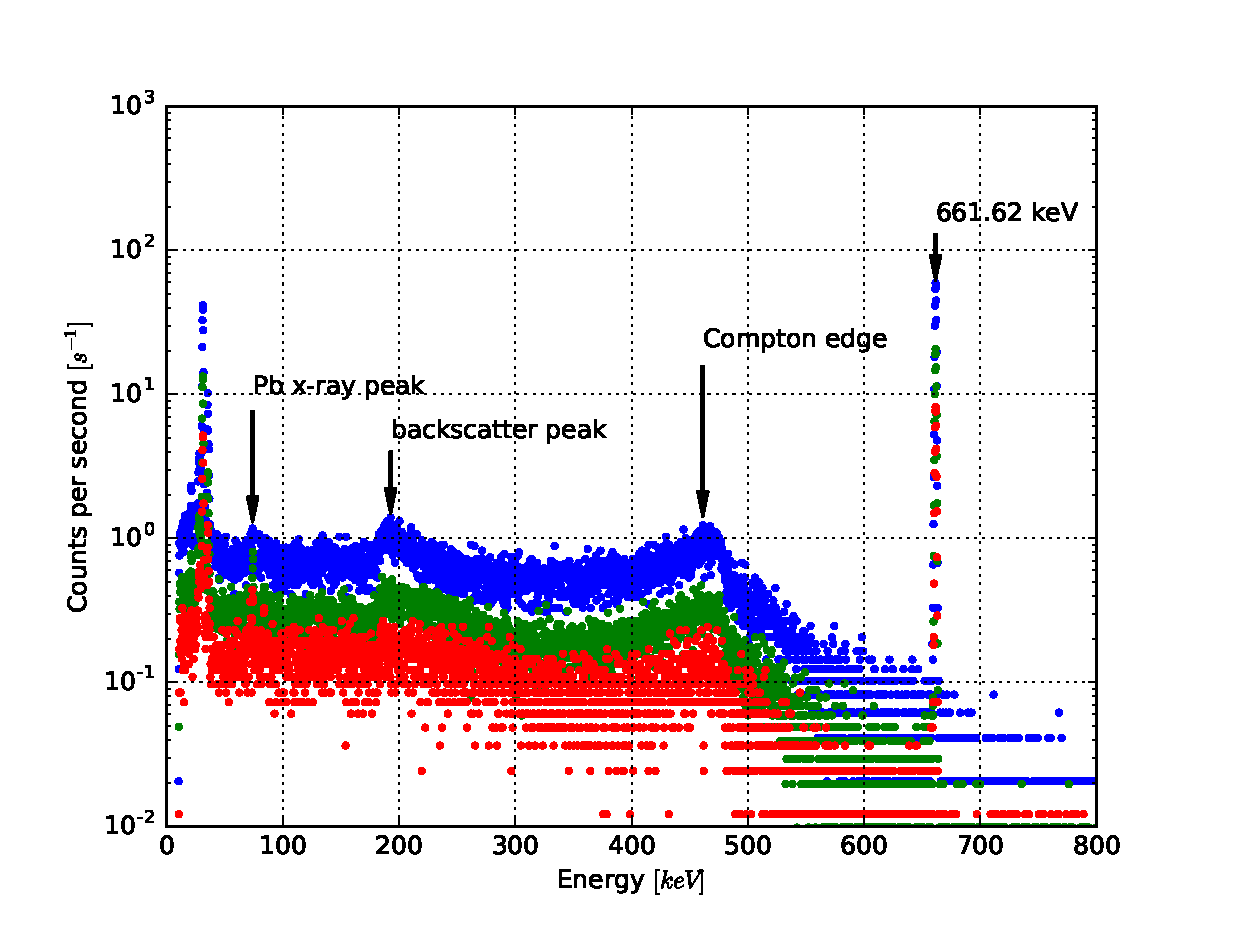
\includegraphics[width=1.0\textwidth]{plots/cs137_ged.eps}
		\end{center}
	\end{minipage}
	\caption{Spectra for $^{137}Cs$; left: $NaI$-detector, right: $Ge$-detector. Source: Authors' own.}
	\label{fig:cs137}
\end{figure}

\subsection{Analysis of the mixed sources}

Figures \ref{fig:gemisch_a} and \ref{fig:gemisch_b} show the spectra of both detectors for the two unknown mixed sources. The scale is chosen to be from $0$ to $1800$ keV, because the highest gamma energy occurring in the samples was $1770.22$ keV for $^{207}Bi$.
\newline
When comparing to the spectra of the known samples, it can be seen that the source called "Gemisch A" has a peak at $661.62$ keV (A), indicating that it contains $^{137}Cs$. This can be seen with both detectors. There are two more peaks (B and C), that can be seen only in the plot of the data from the HPGe detector (right). In the NaI plot (left), these two peaks can only be spotted with much fantasy, and thus barely be indentified as peaks. However this indicates that there is also $^{60}Co$ in the unknown sample, though much less than there is $^{137}Cs$.
\newline
The other sample called "Gemisch B" (figure \ref{fig:gemisch_b}) has similar results. It can be seen in the HPGe plot (right) that the sample contains $^{137}Cs$ (A) as well as $^{60}Co$ (B and C).
\newline
The activity of cesium in "Gemisch B" is higher than in "Gemisch A". Comparing with the known cesium and cobalt source, the activities of both samples are written in table \ref{tab:unknownActivites}. To calculate these activities, the data from the HPGe detector was used.

\begin{figure}[H]
	\begin{minipage}[t]{0.5\textwidth}
		\begin{center}
		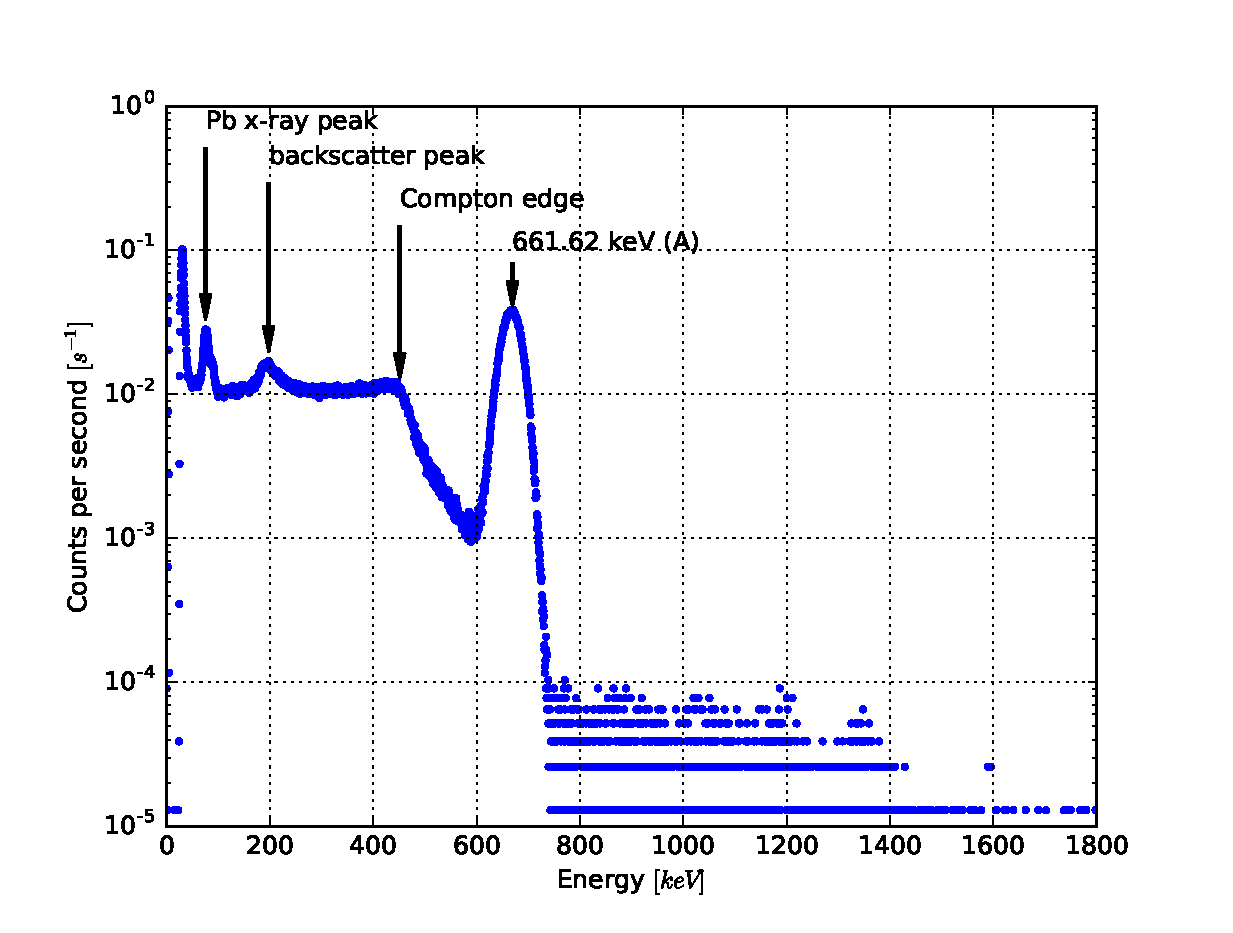
\includegraphics[width=1.0\textwidth]{plots/gemisch_a.eps}
		\end{center}
	\end{minipage}
	\begin{minipage}[t]{0.5\textwidth}
		\begin{center}
		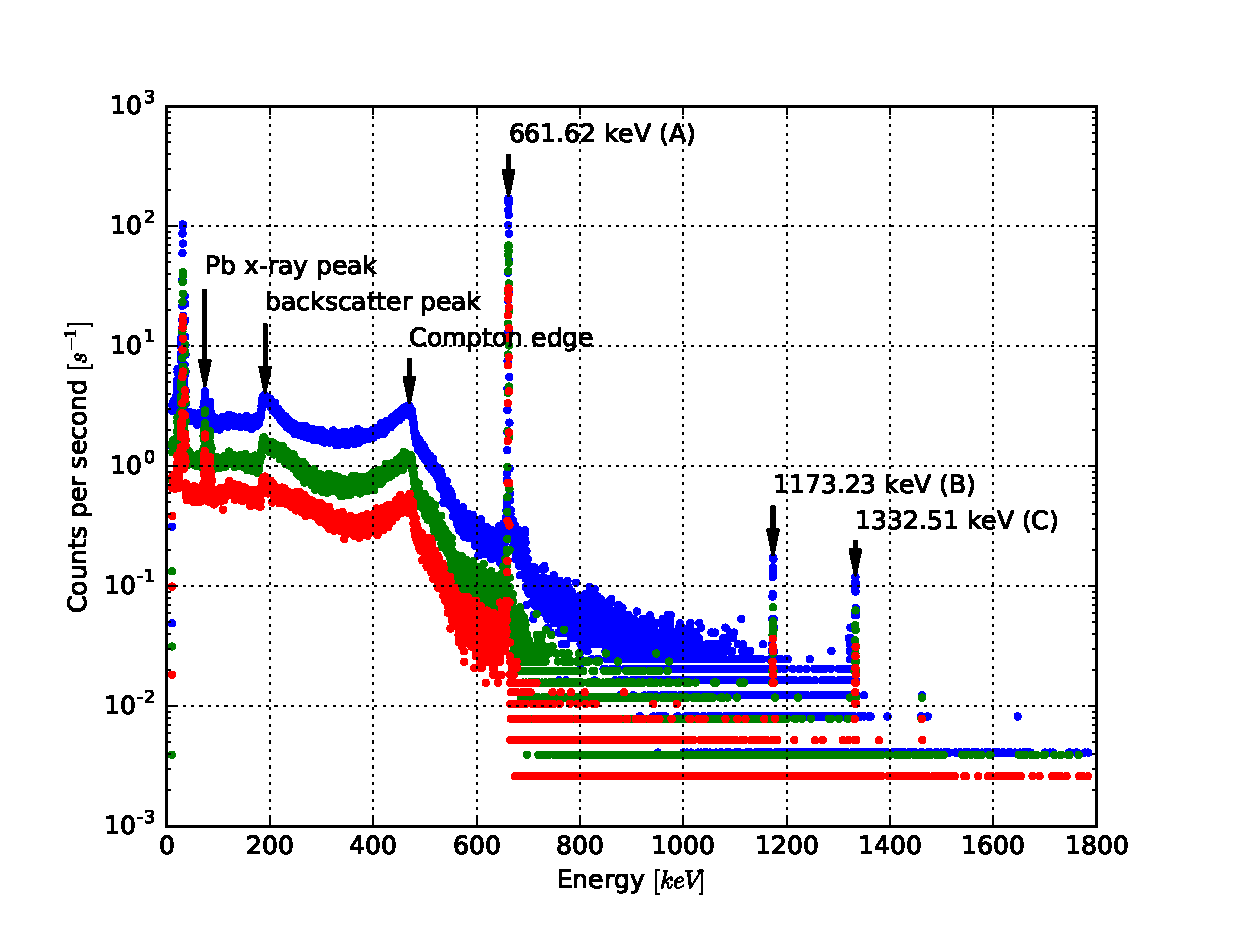
\includegraphics[width=1.0\textwidth]{plots/gemisch_a_ged.eps}
		\end{center}
	\end{minipage}
	\caption{Spectra for Gemisch A; left: $NaI$-detector, right: $Ge$-detector. Source: Authors' own.}
	\label{fig:gemisch_a}
\end{figure}

\begin{figure}[H]
	\begin{minipage}[t]{0.5\textwidth}
		\begin{center}
		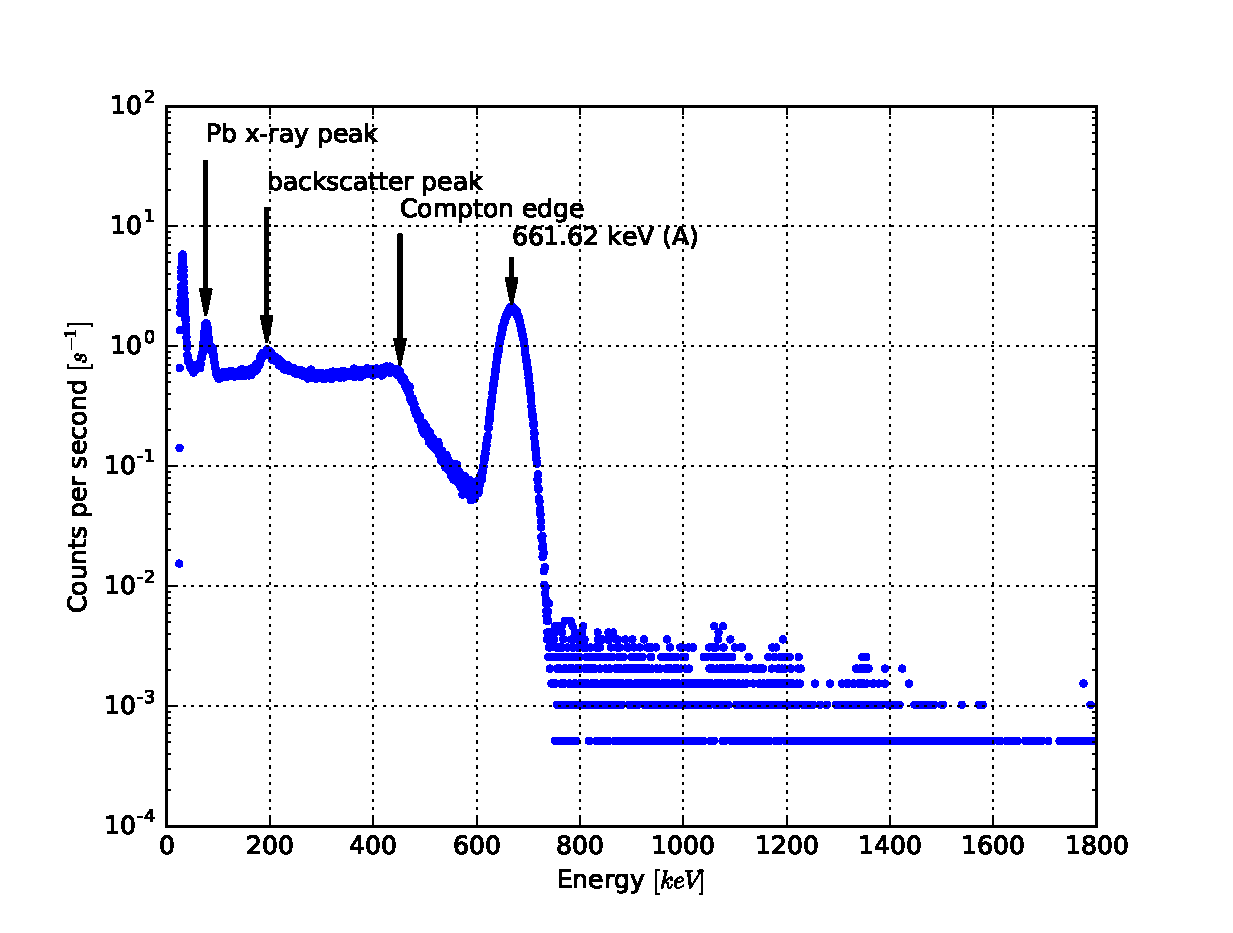
\includegraphics[width=1.0\textwidth]{plots/gemisch_b.eps}
		\end{center}
	\end{minipage}
	\begin{minipage}[t]{0.5\textwidth}
		\begin{center}
		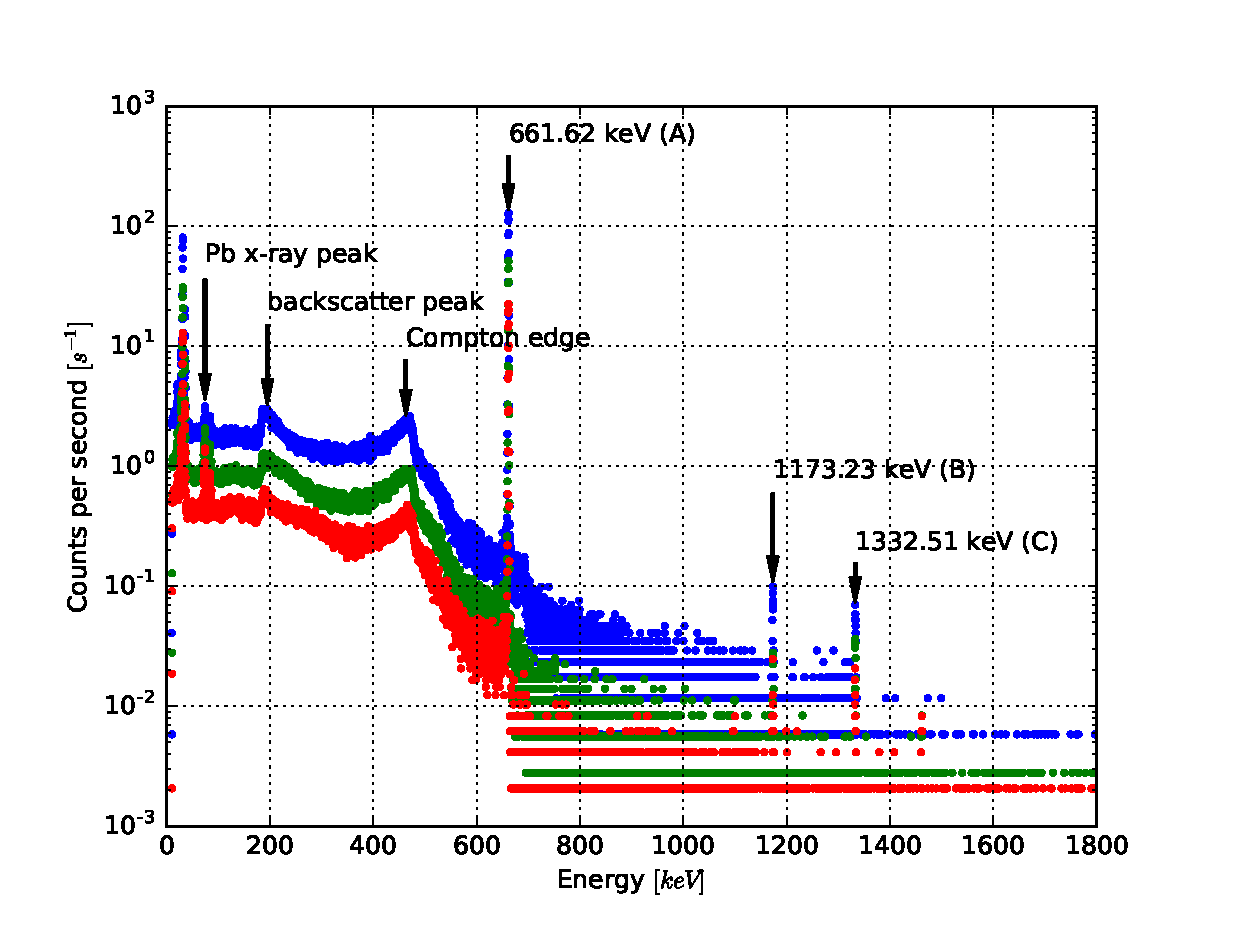
\includegraphics[width=1.0\textwidth]{plots/gemisch_b_ged.eps}
		\end{center}
	\end{minipage}
	\caption{Spectra for Gemisch B; left: $NaI$-detector, right: $Ge$-detector. Source: Authors' own.}
	\label{fig:gemisch_b}
\end{figure}

\begin{table}[H]
\centering
\begin{tabular}{r|rr}
[[tab:unknownActivites]]
\end{tabular}
\caption{Activities of the unknown sources.}
\label{tab:unknownActivites}
\end{table}

\subsection{Analysis of the spectra for $^{152}Eu$}
\label{sec:eu}

In the plots for $^{152}Eu$ (see figure \ref{fig:eu152}), the differences between the two detectors can be seen very well. In both plots many of the photo peaks can be spotted, but the peaks from the HPGe detector (right) are very thin compared to the NaI plots (left). The maxima of the peaks (plotted in counts per second) are much higher in the plot from the HPGe detector compared to the NaI detector (please refer to table \ref{tab:eu152} for all recognizable photo peak values of europium from data of both detectors). This indicates that the HPGe detector is more sensible and therefore detects more gamma-quantums. It is worth mentioning that the ratio between the detected counts per second of both detectors decreases, when the gamma-Energy increases. Hence, the HPGe detector becomes more sensible the higher the energies are (in comparison to the NaI detector).

\begin{figure}[H]
	\begin{minipage}[t]{0.5\textwidth}
		\begin{center}
		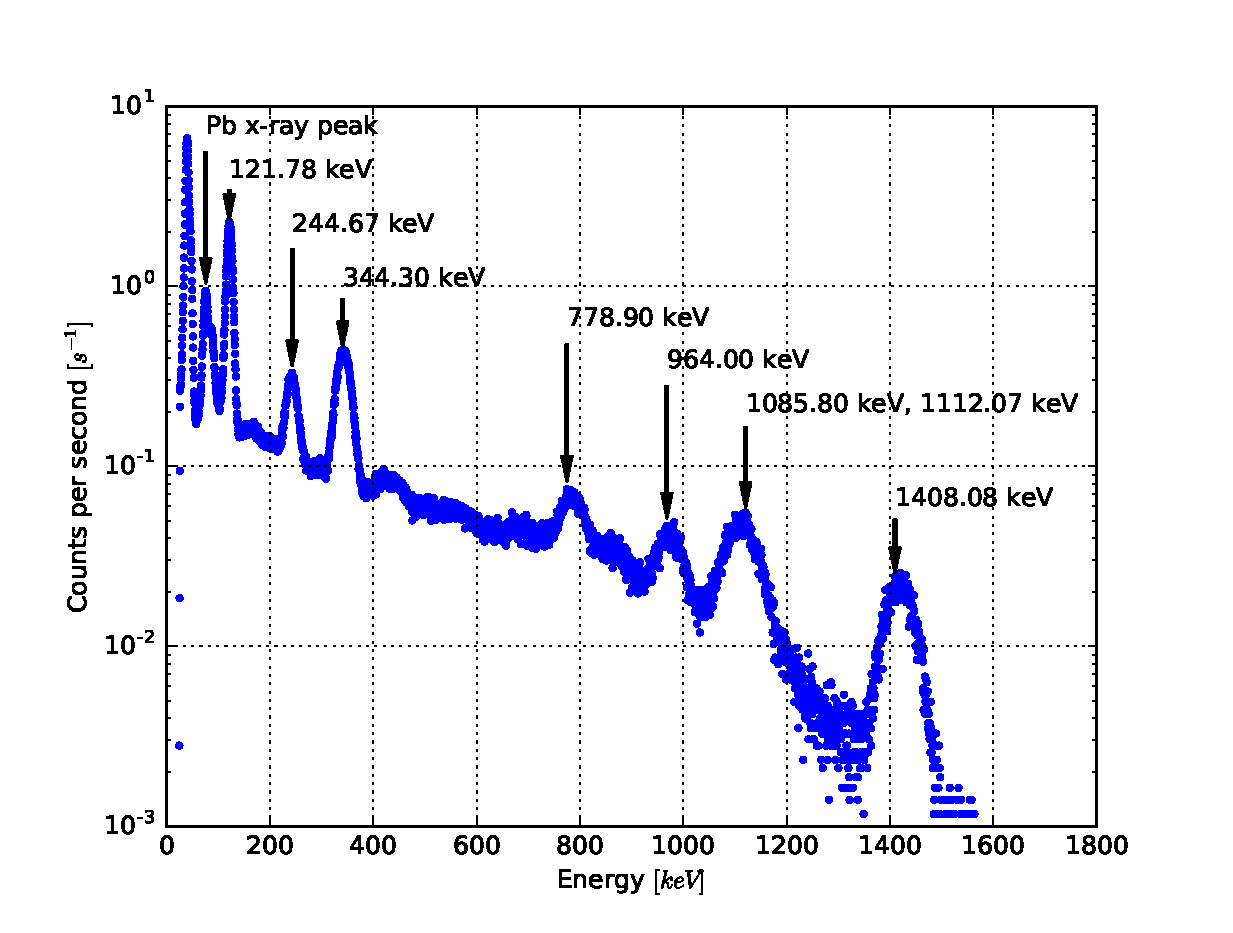
\includegraphics[width=1.0\textwidth]{plots/eu152.eps}
		\end{center}
	\end{minipage}
	\begin{minipage}[t]{0.5\textwidth}
		\begin{center}
		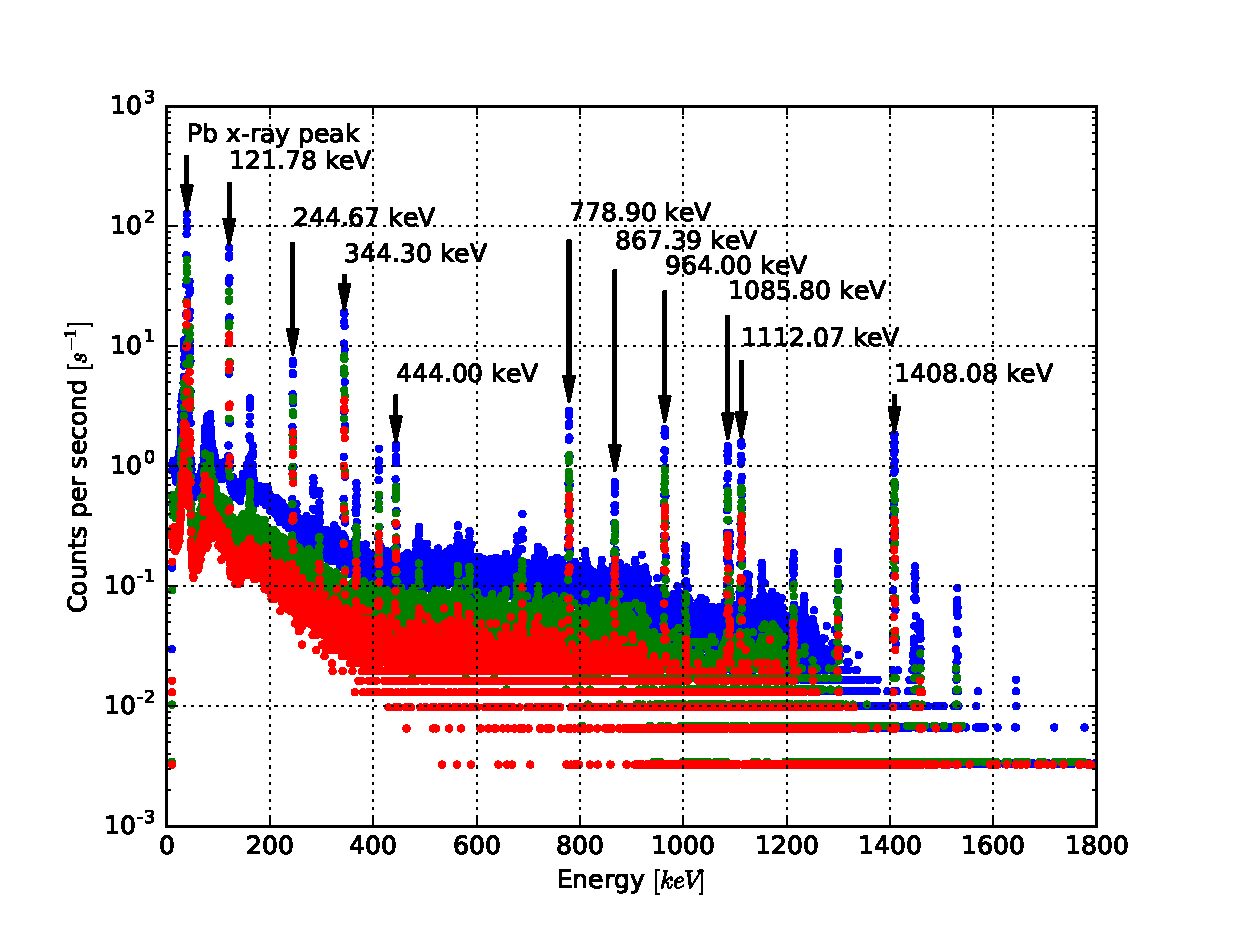
\includegraphics[width=1.0\textwidth]{plots/eu152_ged.eps}
		\end{center}
	\end{minipage}
	\caption{Spectra for $^{152}Eu$; left: $NaI$-detector, right: $Ge$-detector. Source: Authors' own.}
	\label{fig:eu152}
\end{figure}

\begin{table}[H]
\centering
\begin{tabular}{r|rrr}
\hline
[[table:eu152:peaks]]
\end{tabular}
\caption{Calculated data for the maxima of the photo peaks from the spectra of $^{152}Eu$, $c_1$ are the counts per second detected in the NaI detector, $c_2$ are the counts per second detected in the HPGe detector.}
\label{tab:eu152}
\end{table}


\subsection{Errors}

Finding the errors for the measured quantities was in most cases very simple. The computer application MCDWIN already calculated the errors of the channels and energies. All plots of the spectra involve no error bars, because they would be unreadable with them, though the errors would be $\Delta = \sqrt{n}$, where $n$ is the total counts per second of the corresponding channel or energy.
\newline
The error in channels would be $\Delta C = 1$, because this is the scale of the quantity channel.
\newline
Using the error in channels ($\Delta C = 1$), the error in gamma-Energy $\Delta E_{\gamma}$ can be calculated. Since $E_{\gamma}$ is approximately a linear function in $C$ and dependant of the detector, we find:

\begin{subequations}
\begin{align}
\Delta E_{\gamma,NaI} &= [[dE_gamma_NaI]] \ \label{eq:che_a} \\
\Delta E_{\gamma,HPGe} &= [[dE_gamma_HPGe]] \ \label{eq:che_b}
\end{align}
\end{subequations}

These values were obtained using the linear polynomial fits to translate channels into energies. These two fits are as follows:

\begin{subequations}
\begin{align}
p_{NaI}(x) &= [[linear_translation_NaI]] \ \\
p_{HPGe}(x) &= [[linear_translation_HPGe]] \
\end{align}
\end{subequations}

\subsection{Systematic error sources}

In this experiment there are some sources of systematic errors that were neglegted.

\begin{itemize}
\item The channel scale was not perfectly linear to the energy scale, nevertheless a linear interpolation (see equations \eqref{eq:che_a} and \eqref{eq:che_b}) was used to compile channels into energies.
\item The intensity of gamma rays are weakened when penetrating air and matter. This reduction of energy was neglegted in the measurements.
\item All spectra despicted in this report suffer from a small background noise of natural radiation ending up in the detector.
\item The germanium in the HPGe detector has a very high purity, but nonetheless has impurities. These disturb the electric conductivity of the semiconductor. This has an impact to the resolution.
\item In both detectors, not the whole energy of the gamma-quantum is recorded, due to the finite size of the detectors and the fact that in the absorbtion process there is some secondary radiation or scattering occuring, which escapes the detector (for example in the peak of the Compton edge - see figure \ref{fig:cs137} for cesium - the photon will be scattered away from the detector, which results in a reduction of the detected energy; another example is the back-scattering peak).
\item Some emmited gamma rays would not be recognized by the multichannel analyzer, because the aplitude arriving in the oscilloscope is not high enough, thus filtered out. This leads to a systematic error.
\item The photomultiplier has also an efficiency which is not $100 \%$ leading to an error.
\item The integrals to calculate the solid angle correction were only evaluated numerically, not analytically.
\end{itemize}

\subsection{Conclusion}

The comparison between the two detectors (NaI and HPGe) brought up some interessing properties. It seems that the NaI detector is more efficient in detecting high energies, whereas the HPGe detector is more efficient in lower energies. The resolution of the HPGe detector is higher as well. Also the linearity in energy versus channels (the internal scale) is in both detectors given, but in the HPGe detector, the linearity is more strict.

\begin{thebibliography}{9}

\bibitem{hossain2011}
  I. Hossain, N. Sharip and K. K. Viswanathan,
  \textit{Efficiency and resolution of HPGe and NaI(Tl) detectors using gamma-ray spectroscopy},
  Article Number: 8190CA926783,
  pp. 86-89, January 2012,
  Vol.7(1),
  doi: 10.5897/SRE11.1717,
  2011.

\bibitem{flyckt2002}
  S-O Flyckt, C. Marmonier
  \textit{PHOTOMULTIPLIER TUBES - principles \& applications},
  Photonis, Brive, France,
  p 1-2ff,
  September 2002.

\bibitem{lush1965}
  H.J. Lush
  \textit{Photomultiplier linearity},
  Journal of Scientific Instruments,
  Volume 42,
  Number 8,
  1965.

\bibitem{datasheet}
  CANBERRA,
  \textit{Detector specification and performance data (Sheet at the experiment site)},
  GDAME001/F,
  12/03/2007,
  page 1/1,
  2007.

\bibitem{instruction_sheet}
  Ch. Vockenhuber,
  \textit{Versuch: Gamma-Spektroskopie},
  Praktikum für Vorgerückte (VP),
  Instruction Sheet,
  2012.

\bibitem{wiki:semi:2018}
  Wikipedia, [Online],
  \textit{Semiconductor detector},
  November 29, 2018,
  \url{https://en.wikipedia.org/wiki/Semiconductor_detector},

\bibitem{knoll1999}
  Knoll, G.F,
  \textit{Radiation Detection and Measurement},
  3rd ed.,
  Wiley,
  ISBN: 978-0-471-07338-3,
  p 365,
  1999

\bibitem{mcdwin:2018}
  Fast ComTec GmbH, [Online],
  \textit{Multichannel Analyzers},
  December 4, 2018,
  \url{https://www.fastcomtec.com/fwww/datashee/mcd/mcdwin.pdf},

\bibitem{strahlenschutzverordnung}
  Der Schweizerische Bundesrat,
  \textit{Strahlenschutzverordnung (StSV)},
  \url{https://www.admin.ch/opc/de/classified-compilation/20163016/index.html},

\bibitem{akkurt2014}
  I. Akkurt, K. Gunoglu, and S. S. Arda,
  \textit{Detection Efficiency of NaI(Tl) Detector in 511–1332 keV Energy Range},
  StSV,
  Article ID 186798,
  pp. 86-89, January 2012,
  doi: 10.1155/2014/186798,
  2017.

\bibitem{github}
  R. Gruber
  \textit{Source code for the lab report Gamma Spectroscopy},
  2018,
  GitHub repository,
  \url{https://github.com/chaoos/lab-gamma-spectroscopy}.
\end{thebibliography}

\newpage

\section{Appendix}

All measured spectra, not used the discussion above can be found underneath. In all figures of the spectra, the data for the NaI detector is on the left side, whereas the data for the HPGe detector is on the right side. The HPGe detector data are plotted for 3 different lengths in distance to the detector. Blue is $1$ cm in distance from the detector, green $4$ cm and red $8$ cm respectively. The recognizable peaks are labeled and the different photopeaks are labeled with the corresponding gamma energy in keV according \cite{instruction_sheet} (table in section A.4).
\newline
All code used in this report can be found in the GitHub repository \cite{github}.

\begin{figure}[H]
	\begin{minipage}[t]{0.5\textwidth}
		\begin{center}
		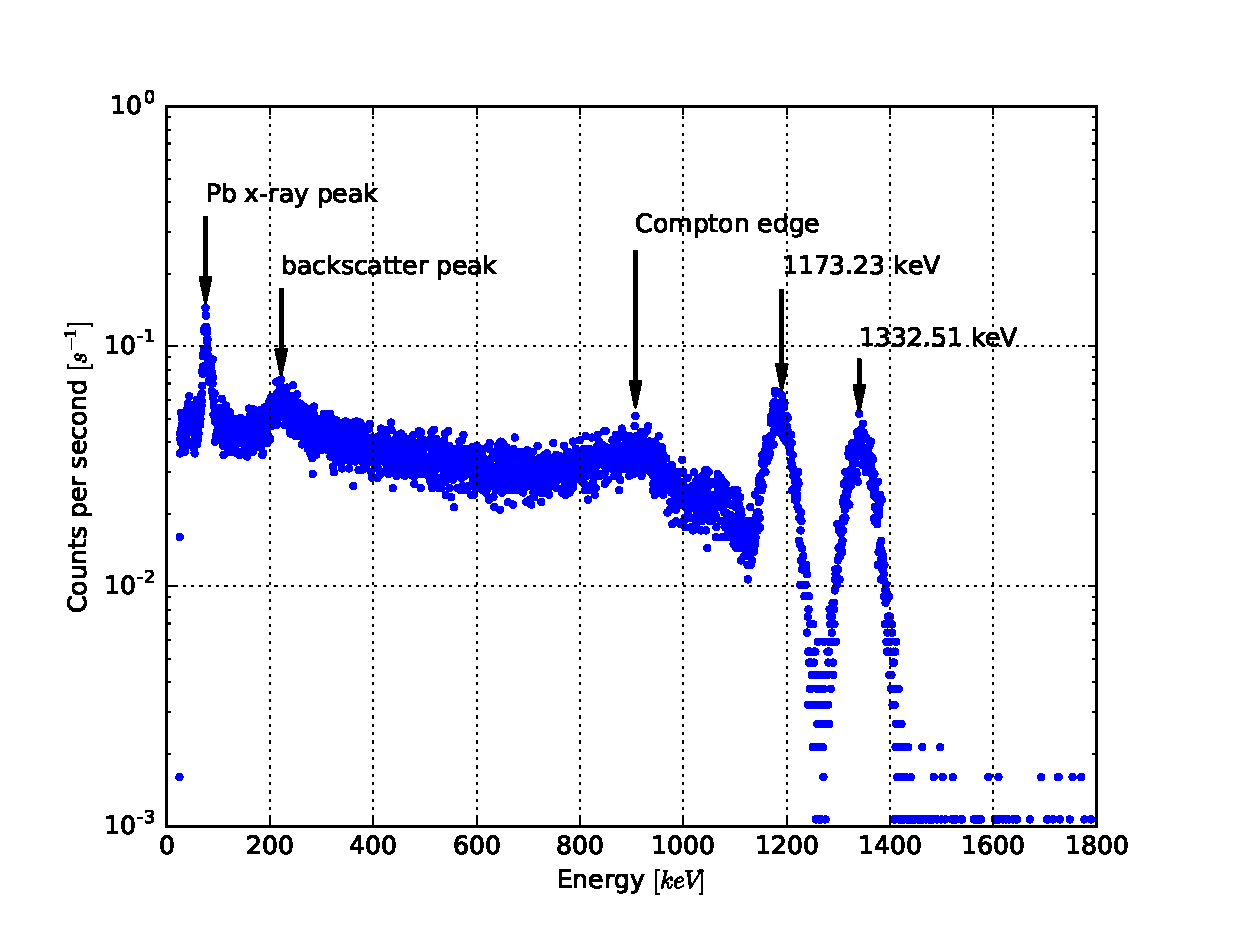
\includegraphics[width=1.0\textwidth]{plots/co60.eps}
		\end{center}
	\end{minipage}
	\begin{minipage}[t]{0.5\textwidth}
		\begin{center}
		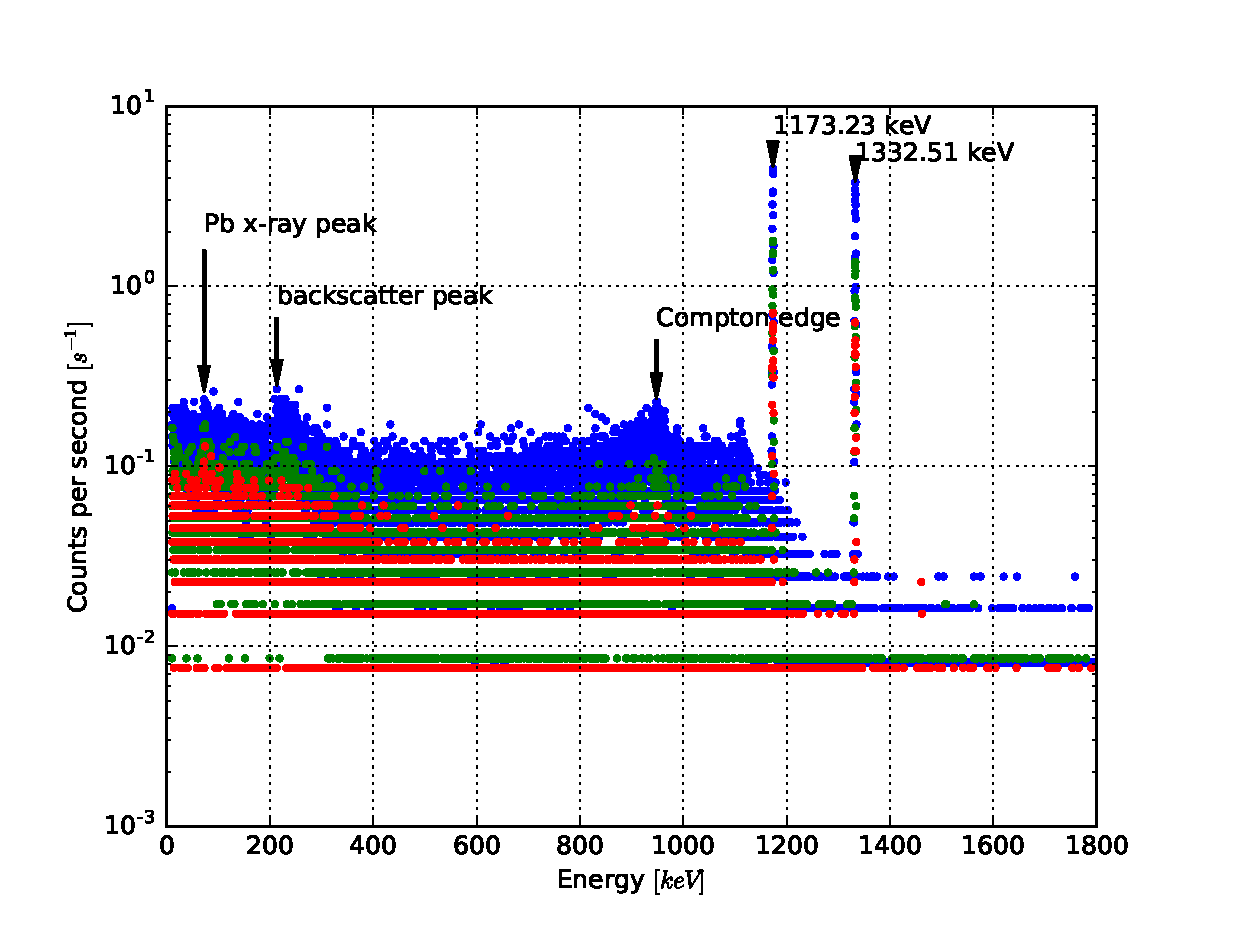
\includegraphics[width=1.0\textwidth]{plots/co60_ged.eps}
		\end{center}
	\end{minipage}
	\caption{Spectra for $^{60}Co$; left: $NaI$-detector, right: $Ge$-detector. Source: Authors' own.}
	\label{fig:co60}
\end{figure}

\begin{figure}[H]
	\begin{minipage}[t]{0.5\textwidth}
		\begin{center}
		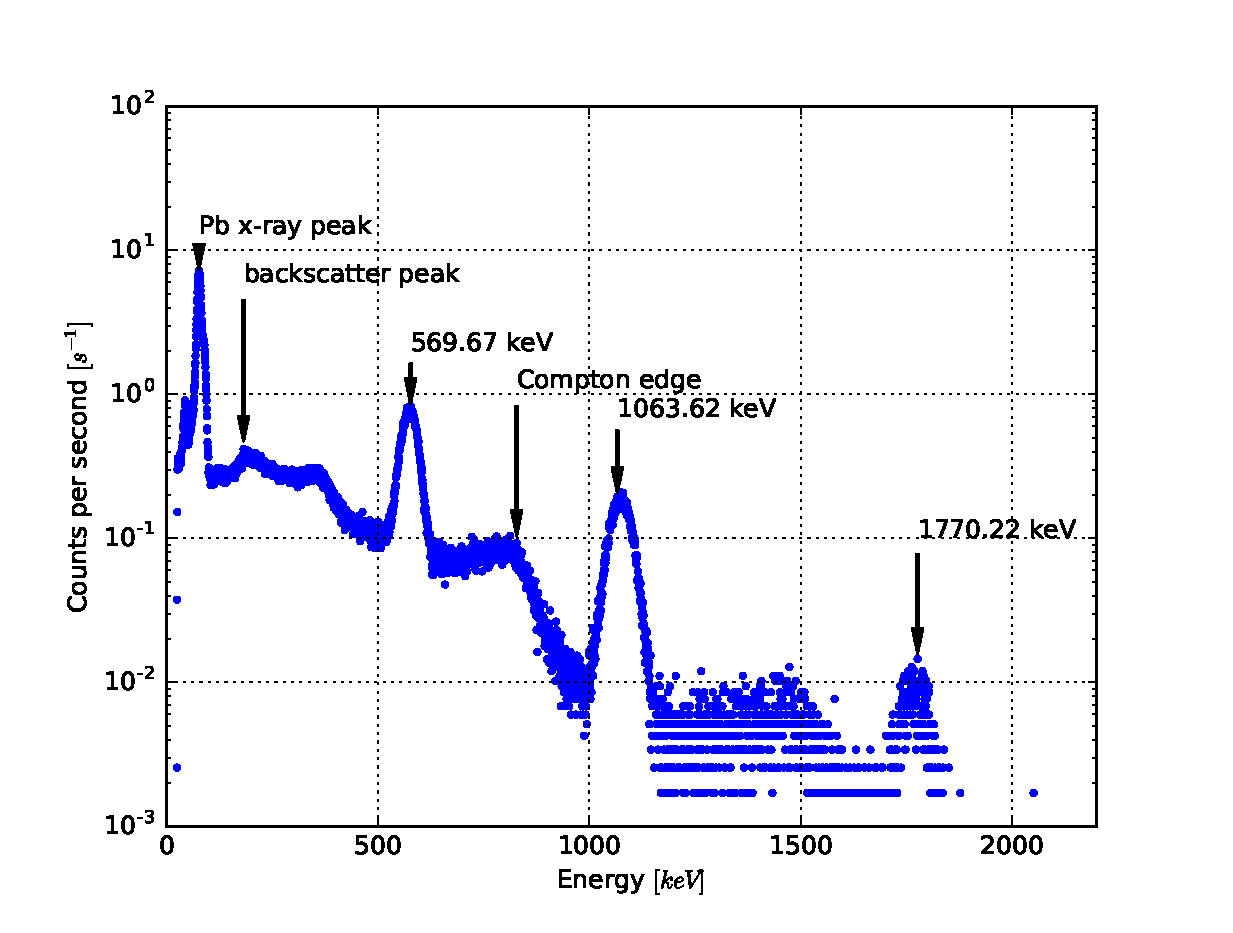
\includegraphics[width=1.0\textwidth]{plots/bi207.eps}
		\end{center}
	\end{minipage}
	\begin{minipage}[t]{0.5\textwidth}
		\begin{center}
		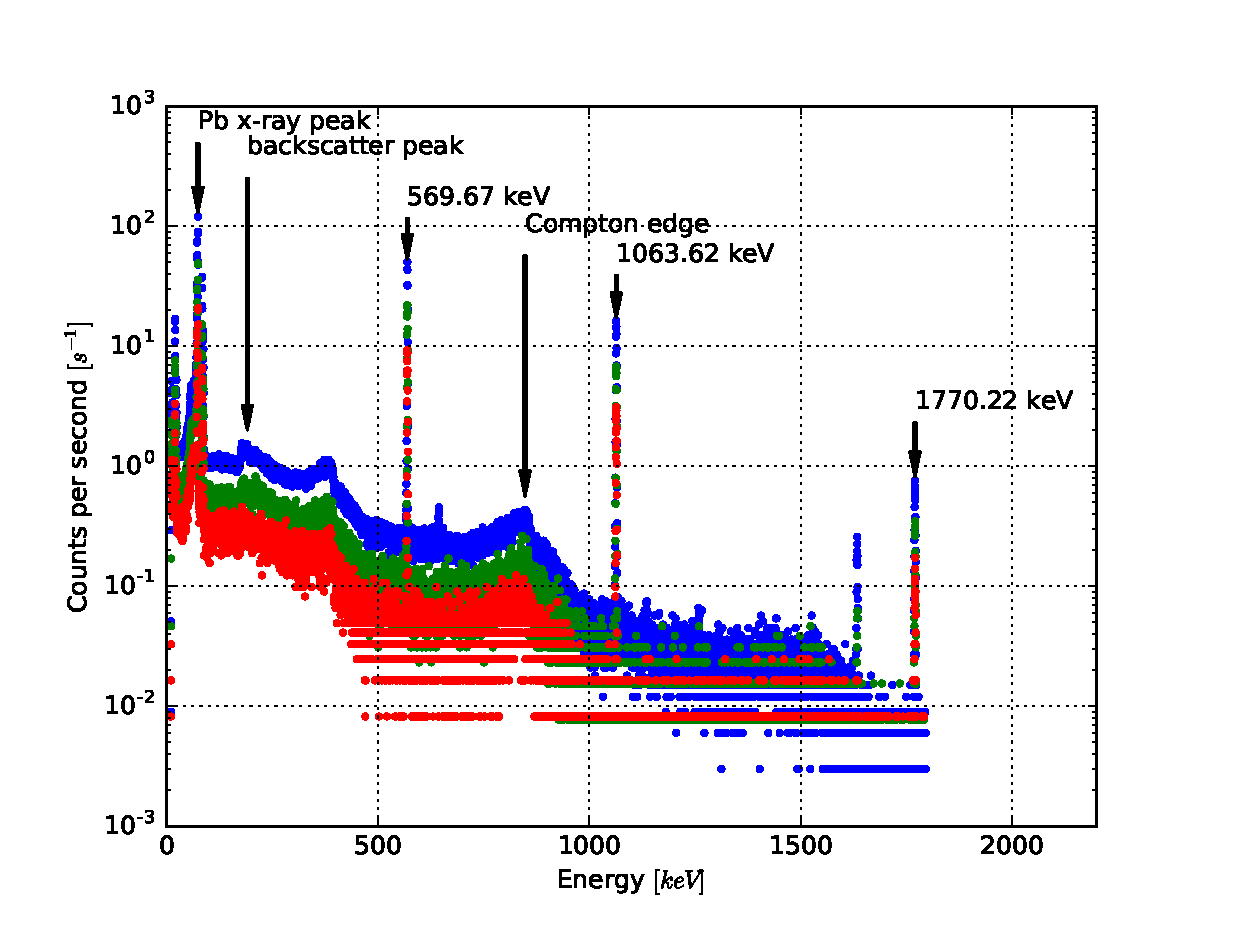
\includegraphics[width=1.0\textwidth]{plots/bi207_ged.eps}
		\end{center}
	\end{minipage}
	\caption{Spectra for $^{207}Bi$; left: $NaI$-detector, right: $Ge$-detector. Source: Authors' own.}
	\label{fig:bi207}
\end{figure}

\begin{figure}[H]
	\begin{minipage}[t]{0.5\textwidth}
		\begin{center}
		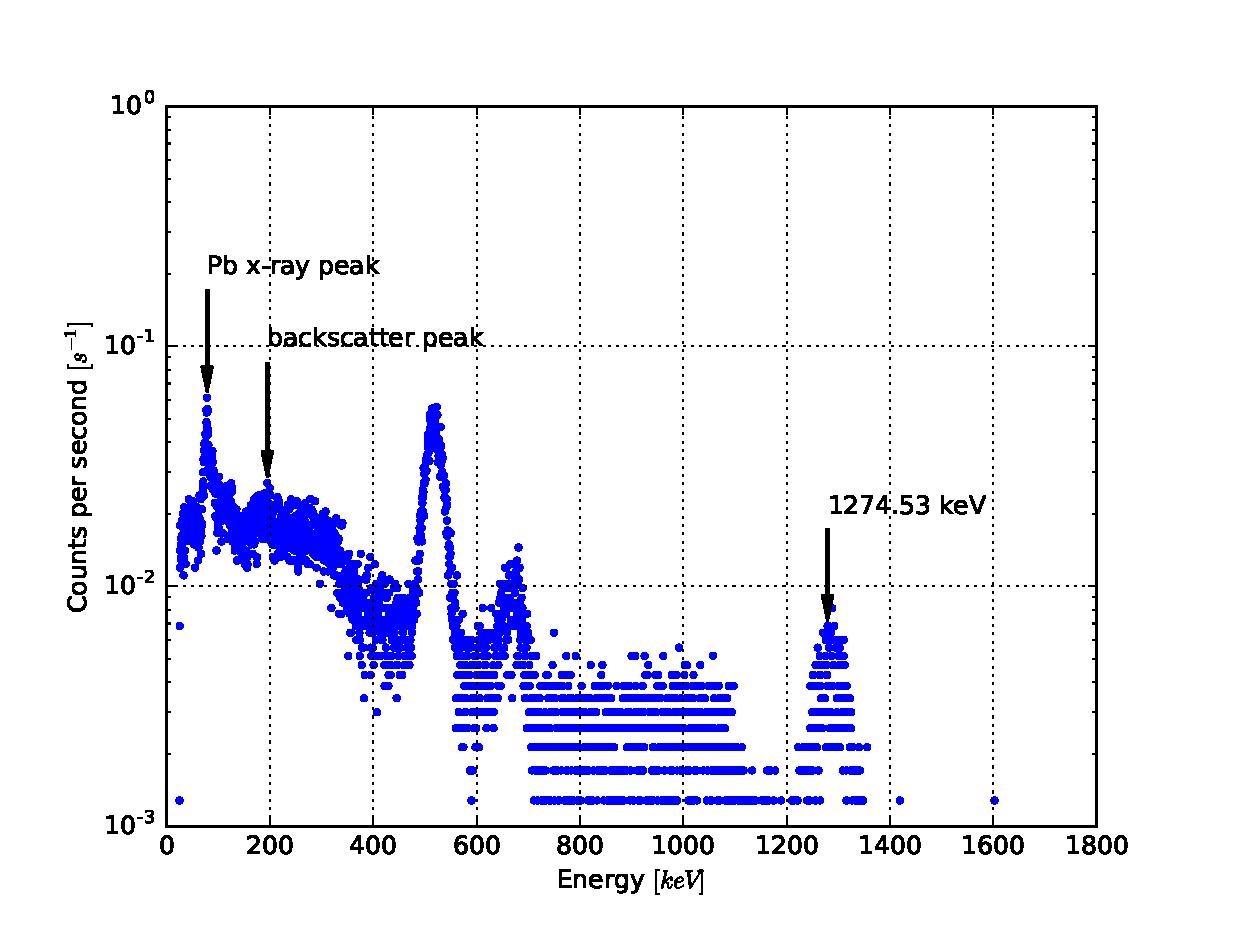
\includegraphics[width=1.0\textwidth]{plots/na22.eps}
		\end{center}
	\end{minipage}
	\begin{minipage}[t]{0.5\textwidth}
		\begin{center}
		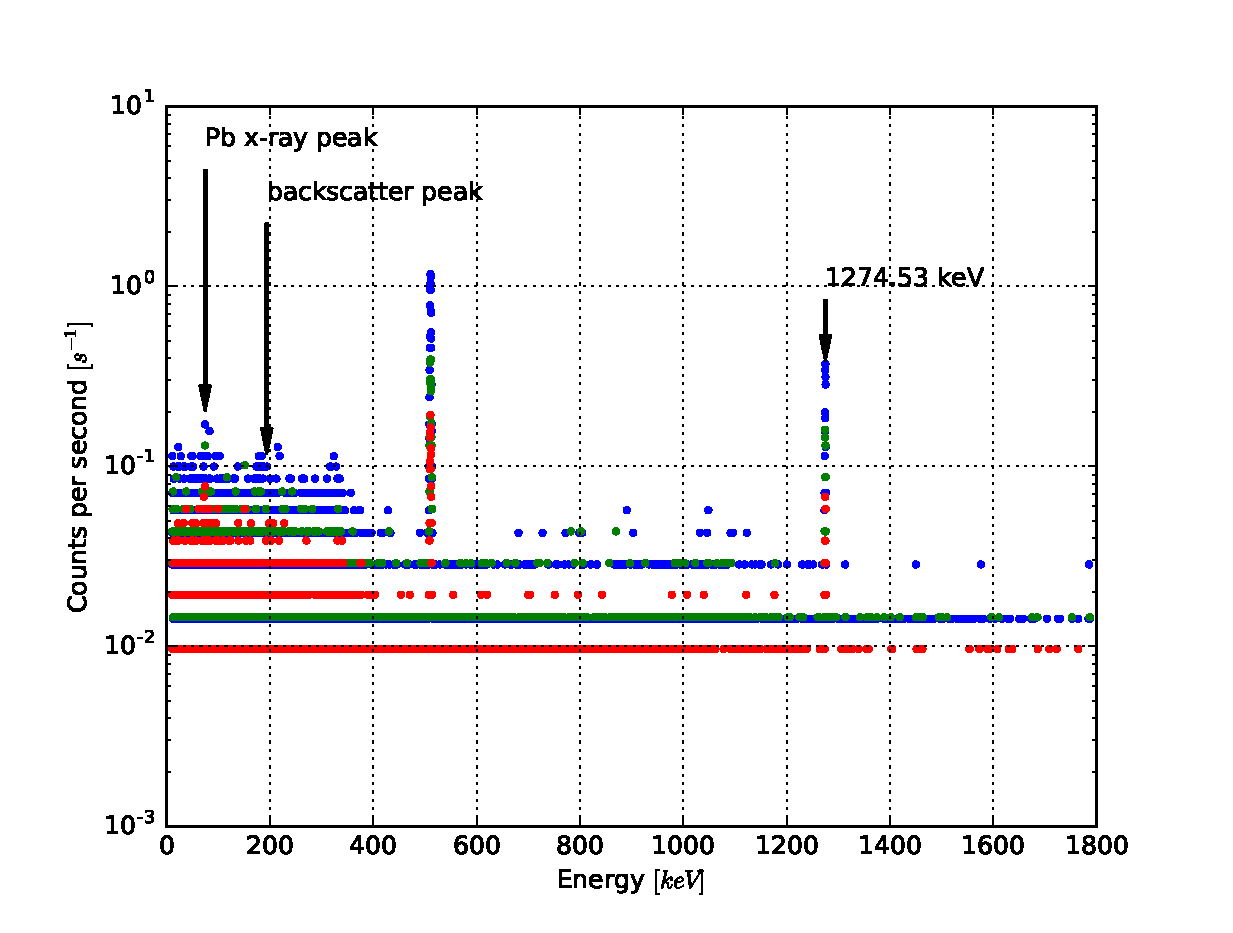
\includegraphics[width=1.0\textwidth]{plots/na22_ged.eps}
		\end{center}
	\end{minipage}
	\caption{Spectra for $^{22}Na$; left: $NaI$-detector, right: $Ge$-detector. Source: Authors' own.}
	\label{fig:na22}
\end{figure}

\begin{table}[H]
\centering
\caption{Measured data for the dose rate.}
\begin{tabular}{r|rrr}
\hline
[[table:doserate]]
\end{tabular}
\label{tab:doserate}
\end{table}

\end{document}